\begin{filecontents*}[overwrite]{\jobname.xmpdata}
\Title{Naslov magistrskega dela} 
\Author{Tina Klobas}
\Keywords{ključna beseda 1\sep ključna beseda 2\sep ključna beseda 3}
\Subject{Fizika}
\end{filecontents*}

%-------------------------------------------------------------------------------------------------

\documentclass[longbibliography,slovene,a4paper,12pt]{book}

%-----------------------------------------------------------------------------------
%     PDF/A
%----------------------------------------------------------------------------------

\usepackage{xmpincl}
\usepackage[a-1b, mathxmp]{pdfx}[2018/12/22]

%-------------------------------------------------------------------------------------

\usepackage[english]{babel}    
\usepackage[utf8]{inputenc}
\usepackage{amsfonts, amsmath}                      %% amsmath for \text{} to work
\usepackage{listings}                               %% for pseudocode
\usepackage[T1]{fontenc}
\usepackage[pdftex]{graphicx}
\usepackage{xcolor,colortbl}
\usepackage{fancyhdr}
\usepackage[explicit,compact]{titlesec}
\titleformat{\chapter}[block]
{\bfseries\huge}{\filright\huge\thechapter.}{1ex}{\huge\filright #1}
\usepackage[sort,numbers]{natbib}
\usepackage[nottoc,numbib]{tocbibind}
\usepackage{acro}
\usepackage{filecontents}
\usepackage{hyperref}
\usepackage{url}
\usepackage[a4paper,inner=3.5cm,outer=2.5cm,top=2.5cm,bottom=2.5cm,pdftex]{geometry}
\usepackage[titletoc, title]{appendix}
\usepackage[outdir=./gnuplot/]{epstopdf}               %% set directory of tex files
\usepackage{makeidx}
\setlength{\headheight}{15pt}
\usepackage{enumitem}
\usepackage{emptypage}
\usepackage{tocloft}
\renewcommand{\cftpartleader}{\cftdotfill{\cftdotsep}} 
\renewcommand{\cftchapleader}{\cftdotfill{\cftdotsep}} 
\usepackage{caption}

\usepackage{standalone}                           %% needed for external tikz files
\usepackage{figures/TikzPack}                     %% needed for external tikz files
\usepackage{gnuplot-lua-tikz}

\def\epsfg#1#2{\epsfig{file=#1.eps,width=#2}}
\def\legendamp#1#2{\vbox{\hsize=#1\caption{\small #2}}}

\setcounter{topnumber}{4}
\setcounter{bottomnumber}{4}
\setcounter{totalnumber}{5}
\renewcommand{\topfraction}{0.99}
\renewcommand{\bottomfraction}{0.99}
\renewcommand{\textfraction}{0.0}
\setlength{\tabcolsep}{10pt}
\renewcommand{\arraystretch}{1.5}

\def\bi#1{\hbox{\boldmath{$#1$}}}
\let\oldvec\vec
\def\vec#1{\mbox{\boldmath$#1$}}
\def\pol{{\textstyle{1\over2}}}
\def\svec#1{\mbox{{\scriptsize \boldmath$#1$}}}

\makeindex
%-----------------------------------------------------------------------------------
%    SUMNIKI
%-----------------------------------------------------------------------------------
%  Za pisanje sumnikov imamo tri moznosti:
%   --- vnasamo jih neposredno v kodnem sistemu UTF-8 (priporocljivo)
%   --- pisemo jih z latexovim ukazom, ki je namenjen natanko temu,
%       in sicer kot \v{c}, \v{s}, \v{z}, \v{C}, \v{S}, v{\Z} ali
%       malo manj pregledno kot \v c, \v s, \v z, \v C, \v S, \v Z,
%   --- pisemo jih kot "c, "s, "z, "C, "S, "Z, vendar tedaj potrebujemo
%       spodaj zapisani macro, ki znaku " pripise vlogo `izdelave' sumnika:
\catcode`\"=\active\def"#1{\v{#1}}
%       torej \v{S}krjan\v{c}ek == \v Skrjan\v cek == "Skrjan"cek
%  Pozor: narekovaj potem ne smemo vec pisati kot " ampak kot `` in ''
%       torej: "Skrjan"cek je "civkal ``"ci-"ci-"ci''.

\newcommand{\e}{\mathrm{e}}

%-----------------------------------------------------------------------------------
%   PRIPOROCILO
%
%  V primeru, da je besedilna datoteka prevelika za pregledno urejanje,
%  priporocamo, da vsebino razdelite na posamezna poglavja, ki jih v glavni
%  dokument vkljucite z ukazom \input{naslov_poglavja}.
%
%-----------------------------------------------------------------------------------

%% dodam svoje barve, da bojo povsod enake
% \definecolor{myblue}{HTML}{043565}
% \definecolor{mymagenta}{HTML}{8f2d56}
% \definecolor{myteal}{HTML}{218380}
% \definecolor{mytangerine}{HTML}{fb9f89}
% \definecolor{mygray}{HTML}{9a9aac}
% \definecolor{myyellow}{HTML}{ffc43d}

\definecolor{myred}{HTML}{f94144}
\definecolor{myredorange}{HTML}{f3722c}
\definecolor{myorange}{HTML}{f8961e}
\definecolor{myyellow}{HTML}{f9c74f}
\definecolor{mylightgreen}{HTML}{90be6d}
\definecolor{mygreen}{HTML}{43aa8b}
\definecolor{myblue}{HTML}{577590}

\begin{document}

%-----------------------------------------------------------------------------------
%       NASLOVNA STRAN 
%-----------------------------------------------------------------------------------

\pagestyle{empty}
\begin{center}

{\large UNIVERZA V LJUBLJANI\\
 FAKULTETA ZA MATEMATIKO IN FIZIKO\\
ODDELEK ZA FIZIKO\\
FIZIKA II.~STOPNJA, FIZIKA KONDENZIRANE SNOVI\\}


\vspace{4cm}
{\Large Tina Klobas\\}
\vspace{10mm}
{\bf \Large ORIENTACIJSKO ZAGOZDENJE DVODIMENZIOALNIH ELIPS V RAVNINI}\\
\vspace{5mm}
{\large Magistrsko delo}\\

\vfill

{\large MENTOR: dr. Anže Božič\\
SOMENTOR: doc. dr. Simon Čopar\\

\vspace{2cm}
Ljubljana, 2023}

\end{center}

%-----------------------------------------------------------------------------------
%        ZAHVALA (NEOBVEZNO)
%-----------------------------------------------------------------------------------

% \cleardoublepage
% \mbox{}
% \vfill
% {\Large \bf Zahvale}
% \vspace{1cm}\\
% Na tem mestu zapi"site, komu se zahvaljujete za pomo"c pri nastanku magistrskega 
% dela.

%-----------------------------------------------------------------------------------
%         IZVLECEK
%-----------------------------------------------------------------------------------

% \cleardoublepage
\pagestyle{plain}
\begin{center}
{\bf Naslov v slovenskem jeziku}\\[3mm]
{\sc  Izvle"cek}
\end{center}
\vspace{10mm}
Kratek izvle"cek v slovenskem jeziku, do 300 besed.\\[10mm]
{\bf Klju"cne besede:}\\[3mm]


\cleardoublepage
\foreignlanguage{english}{  %  angleski delilni vzorci
\begin{center}
{\bf Naslov v angleškem jeziku}\\[3mm]
{\sc  Abstract}
\end{center}
\vspace{10mm}
Kratek izvleček v angleškem jeziku, do 300 besed.\\[10mm]
{\bf Keywords:}\\[3mm]
}

%-----------------------------------------------------------------------------------
%    KAZALO
%-----------------------------------------------------------------------------------

% \cleardoublepage
% \tableofcontents

%-----------------------------------------------------------------------------------
%       OSREDNJI DEL
%-----------------------------------------------------------------------------------

\cleardoublepage
\pagestyle{headings}
\fancyhead[CE,RE]{}
\fancyhead[LO,CO]{}
\fancyhead[LE]{\textbf{\nouppercase{\leftmark}}}
\fancyhead[RO]{\textbf{\nouppercase{\rightmark}}}


%\chapter{Uvod}
\label{chUvo}

Zelo pomemben je jezik ter razumljivost pisanja. Besedilo mora biti pripravljeno 
v skladu s pravili za objavo v znanstveni reviji.  Nekaj koristnih nasvetov 
o strokovnem pisanju najdete v "clanku prof. Ivana Ku"s"cerja : O strokovnem pisanju 
\cite{Ku}.  Pomagate si lahko tudi z navodili Ameri"skega fizikalnega dru"stva 
\cite{APS}.\\

Vse strani morajo biti "stete, tudi prazne strani, priloge med besedilom in na koncu 
dela.  Osrednje besedilo mora biti o"stevil"ceno z arabskimi "stevilkami, za"cetne 
in kon"cne strani pa so lahko o"stevil"cene tudi z rimskimi "stevilkami.  "Stevilke 
morajo biti izpisane na spodnjem delu strani. Tisk naj bo razen za"cetnih strani 
dvostranski.  Obvezna je vezava v trde platnice.\\

{\bf Vrstni red vsebine:}

\begin{itemize}[noitemsep]
\item{Naslovna stran}
\item{Zahvala (neobvezno)}
\item{Izvle"cek v slovenskem jeziku. Dodajte tudi klju"cne besede v slovenskem jeziku}
\item{Izvle"cek v angle"skem jeziku. Dodajte tudi klju"cne besede v angle"skem jeziku}
\item{Kazalo vsebine}
\item{Uvod}
\item{Osrednji del}
\item{Zaklju"cni del}
\item{Seznam literature}
\item{Dodatki (neobvezno)}
\item{Stvarno kazalo (neobvezno)}
\end{itemize}

Literatura mora biti citirana "ze v besedilu. Citirani viri sproti povedo, kje naj 
bralec i"s"ce dodatne informacije.  Seznam naj bo urejen po vrstnem redu, kot se 
navedbe pojavijo v delu.  V primeru uporabe programa {Bib\TeX} za navajanje literature 
izberite Bib\TeX{ov} stil, prirejen po apsrev4-2.bst, ki ga najdete na spletni strani 
poleg te predloge.  Navodila za delo s programom {Bib\TeX} najdete na spletni strani 
\cite{Bib}, navodila za namestitev paketa REVTeX 4.1 pa na strani \cite{Rev}.  Za vnos 
bibliografskih enot priporo"camo uporabo programa \href{http://www.jabref.org/}{JabRef} 
\cite{JR}.  V seznamu literature te predloge smo naslove spletnih strani in online 
dokumentov vnesli v polje {\tt Note} pred datumom ogleda spletne strani.  "Ce "zelite, 
da se vam v seznamu literature elektronski naslov ne izpi"se, ga vnesite v polje 
{\tt URL}.  V vseh primerih, kjer je to mo"zno, dodajte aktivne povezave za dostop 
do elektronskih dokumentov.  Pred izpolnjevanjem polj obvezno preberite navodila 
v pomo"ci (User Documentation). Tu je izsek iz navodil: 
\href{https://docs.jabref.org/advanced/fields}{About BibTeX and its fields} \cite{Help}.\\

\index{Bib\TeX}
\lstset{language=Python}
\lstset{frame=tb,
  language=Python,
  aboveskip=3mm,
  belowskip=3mm,
  showstringspaces=false,
  columns=flexible,
  basicstyle={\small\ttfamily},
  numbers=none,
  numberstyle=\tiny\color{gray},
  keywordstyle=\color{myteal},
  commentstyle=\color{myblue},
  stringstyle=\color{myyellow},
  breaklines=true,
  breakatwhitespace=true,
  tabsize=3
}

\chapter{Metodologija}
\label{chMe}
Okviren potek zagozdenja sistema:
\begin{enumerate}
\item Z Mitchellovim algoritmom~\cite{mitch} ustvarimo dvodimenzionalno mrežo z $N$ 
    točkami.
\item Točke postanejo središča elips z~ekscentričnostjo $e$ in naključnimi začetnimi 
    orientacijami.
\item Implementacija prekrivalne funkcije~\cite{perram1985} za zaznavanje trkov med 
    elipsami.
\item Postopno večanje elips in relaksacija vrtenja (Monte Carlo).
\item Analiza konfiguracij.
\end{enumerate}
Periodične robne pogoje v~kodi implementiramo na naslednji način
\begin{lstlisting}[frame=single]  
    dx = point2 - point1
    if dx > 0.5*width:
        dx = dx - width
    elif dx < -0.5*width:
        dx = dx + width
\end{lstlisting}

\section{Mitchellov algoritem}
Okviren potek algoritma:
\begin{enumerate}
    \item Postavimo začetni točki na naključna položaja.
    \item Zgeneriramo naključne položaje kandidatov za naslednjo točko.
    \item Izberemo kandidata, ki je najdlje od vseh točk porazdelitve 
    (ima največjo minimalno oddaljenost).
    \item Ponavljamo prejšnje korake dokler ne dosežemo izbranega števila točk.
\end{enumerate}
Na vsaki ponovitvi število kandidatov povečamo sorazmerno s~številom že 
obstoječih točk $n$. Pri nalogi smo tako vsakič generirali 
$ \left \lfloor{n/2}\right \rfloor + 1$ kandidatov.\\
%% napisi se nek del kako je to kul in primerjavo z modrim sumom blabla
Primer za porazdelitev $1024$ točk je prikazana na sliki~\ref{fig:porazdelitev_tock}.
Zdaj v~točke postavimo elipse enakih velikosti ($a$, $b$ in $e$) in naključnih
orientacij $\theta_i$. Potrebujemo še kriterij za zaznavanje prekritih elips,
kar je predstavljeno v~naslednjem razdelku.
\begin{figure}[!ht]
    \centering
    \resizebox{.7\textwidth}{!}{% GNUPLOT: LaTeX picture with Postscript
\begingroup
  \makeatletter
  \providecommand\color[2][]{%
    \GenericError{(gnuplot) \space\space\space\@spaces}{%
      Package color not loaded in conjunction with
      terminal option `colourtext'%
    }{See the gnuplot documentation for explanation.%
    }{Either use 'blacktext' in gnuplot or load the package
      color.sty in LaTeX.}%
    \renewcommand\color[2][]{}%
  }%
  \providecommand\includegraphics[2][]{%
    \GenericError{(gnuplot) \space\space\space\@spaces}{%
      Package graphicx or graphics not loaded%
    }{See the gnuplot documentation for explanation.%
    }{The gnuplot epslatex terminal needs graphicx.sty or graphics.sty.}%
    \renewcommand\includegraphics[2][]{}%
  }%
  \providecommand\rotatebox[2]{#2}%
  \@ifundefined{ifGPcolor}{%
    \newif\ifGPcolor
    \GPcolortrue
  }{}%
  \@ifundefined{ifGPblacktext}{%
    \newif\ifGPblacktext
    \GPblacktexttrue
  }{}%
  % define a \g@addto@macro without @ in the name:
  \let\gplgaddtomacro\g@addto@macro
  % define empty templates for all commands taking text:
  \gdef\gplbacktext{}%
  \gdef\gplfronttext{}%
  \makeatother
  \ifGPblacktext
    % no textcolor at all
    \def\colorrgb#1{}%
    \def\colorgray#1{}%
  \else
    % gray or color?
    \ifGPcolor
      \def\colorrgb#1{\color[rgb]{#1}}%
      \def\colorgray#1{\color[gray]{#1}}%
      \expandafter\def\csname LTw\endcsname{\color{white}}%
      \expandafter\def\csname LTb\endcsname{\color{black}}%
      \expandafter\def\csname LTa\endcsname{\color{black}}%
      \expandafter\def\csname LT0\endcsname{\color[rgb]{1,0,0}}%
      \expandafter\def\csname LT1\endcsname{\color[rgb]{0,1,0}}%
      \expandafter\def\csname LT2\endcsname{\color[rgb]{0,0,1}}%
      \expandafter\def\csname LT3\endcsname{\color[rgb]{1,0,1}}%
      \expandafter\def\csname LT4\endcsname{\color[rgb]{0,1,1}}%
      \expandafter\def\csname LT5\endcsname{\color[rgb]{1,1,0}}%
      \expandafter\def\csname LT6\endcsname{\color[rgb]{0,0,0}}%
      \expandafter\def\csname LT7\endcsname{\color[rgb]{1,0.3,0}}%
      \expandafter\def\csname LT8\endcsname{\color[rgb]{0.5,0.5,0.5}}%
    \else
      % gray
      \def\colorrgb#1{\color{black}}%
      \def\colorgray#1{\color[gray]{#1}}%
      \expandafter\def\csname LTw\endcsname{\color{white}}%
      \expandafter\def\csname LTb\endcsname{\color{black}}%
      \expandafter\def\csname LTa\endcsname{\color{black}}%
      \expandafter\def\csname LT0\endcsname{\color{black}}%
      \expandafter\def\csname LT1\endcsname{\color{black}}%
      \expandafter\def\csname LT2\endcsname{\color{black}}%
      \expandafter\def\csname LT3\endcsname{\color{black}}%
      \expandafter\def\csname LT4\endcsname{\color{black}}%
      \expandafter\def\csname LT5\endcsname{\color{black}}%
      \expandafter\def\csname LT6\endcsname{\color{black}}%
      \expandafter\def\csname LT7\endcsname{\color{black}}%
      \expandafter\def\csname LT8\endcsname{\color{black}}%
    \fi
  \fi
    \setlength{\unitlength}{0.0500bp}%
    \ifx\gptboxheight\undefined%
      \newlength{\gptboxheight}%
      \newlength{\gptboxwidth}%
      \newsavebox{\gptboxtext}%
    \fi%
    \setlength{\fboxrule}{0.5pt}%
    \setlength{\fboxsep}{1pt}%
    \definecolor{tbcol}{rgb}{1,1,1}%
\begin{picture}(7200.00,5040.00)%
    \gplgaddtomacro\gplbacktext{%
    }%
    \gplgaddtomacro\gplfronttext{%
    }%
    \gplbacktext
    \put(0,0){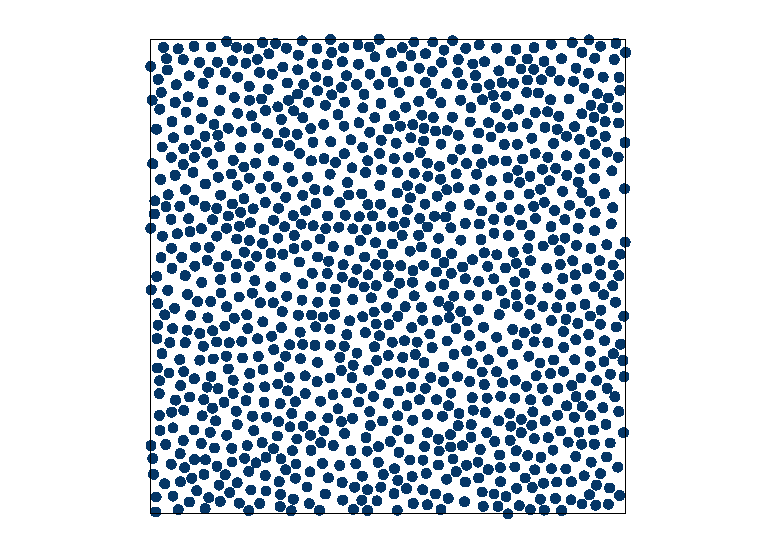
\includegraphics[width={360.00bp},height={252.00bp}]{./gnuplot/porazdelitev_1024}}%
    \gplfronttext
  \end{picture}%
\endgroup
}
    \caption[Blue noise]{Porazdelitev $1024$ točk.}
    \label{fig:porazdelitev_tock}
\end{figure}

\section{Eliptična kontaktna funkcija}
Za zaznavanje prekrivanja para elips implementiramo kontaktno funkcijo, povzeto
po~\cite{perram1985}.

\subsection{Ena elipsa}
Elipsa $A$ je definirana s~centrom $\vec{r}_A$, orientacijo $\theta_A$ in pozitivno 
definitno kvadratično formo $\mathbf{A}$ kot množica točk, za katero velja
\begin{equation}
    E_A (\vec{r}-\vec{r}_A, \theta_A) = 
    (\vec{r} - \vec{r}_A)^{\top} \mathbf{A}^{-1} (\vec{r} - \vec{r}_A)
    \begin{cases}
        \quad <1 & \text{znotraj A},\\
        \quad =1 & \text{na površini A},\\
        \quad >1 & \text{zunaj A}.
    \end{cases}
    \label{eq:elipsa}
\end{equation}
Z~uporabo rotacijske matrike $R(\theta)$ lahko $\mathbf{A}$ zapišemo kot
\begin{equation}
    \mathbf{A} (\theta_A) = \mathbf{R}(\theta_A) \hat{\mathbf{A}} 
                            \mathbf{R}^{\top}(\theta_A).
\end{equation}
Kjer je $\hat{\mathbf{A}}$ določena z~velikostjo polosi elipse $a_1$ in $a_2$ 
ter enotskih vektorjev $\vec{e}_i$ 
\begin{equation}
    \hat{\mathbf{A}} = \sum_{i=1}^{2} a_i^2 \vec{e}_i \vec{e}_i^{\top}.
\end{equation}

\subsection{Prekrivanje dveh elips}
Definiramo funkcijo
\begin{equation}
    F(\vec{r}, \lambda) = \lambda E_A (\vec{r}) + (1 - \lambda) E_B (\vec{r}),
    \label{eq:F}
\end{equation}
kot vsoto dveh elips $A$ in $B$, ter izbranega parametra $\lambda$. Tega omejimo na
interval $[0,1]$ tako, da je $F(\vec{r}, \lambda) \geq 0$. Pri fiksni vrednosti 
$\lambda$ ima $F(\vec{r}, \lambda)$ enolični minimum. 
Za skrajni vrednosti lahko trivialno zaključimo, da je minimum $F=0$ pri 
$\vec{r} = \vec{r}_B$ za $\lambda=0$ oziroma pri $\vec{r} = \vec{r}_A$ za 
$\lambda=1$. 
Za vse vmesne vrednosti $\lambda$ lego minimuma $\vec{r}$ dobimo z~minimizacijo.
Sledi
\begin{equation}
    \nabla F(\vec{r}, \lambda) = 0,
\end{equation}
oziroma
\begin{equation}
    \lambda \mathbf{A}^{-1} (\vec{r} - \vec{r}_A) + (1-\lambda) \mathbf{B}^{-1}
    (\vec{r} - \vec{r}_B) = 0.
    \label{eq:min_F}
\end{equation}
Rešitev minimizacije je pot $\vec{r}(\lambda)$ med centroma elips, ki jo lahko izrazimo 
iz enačbe~\ref{eq:min_F} kot sistem
\begin{align}
    \vec{r}(\lambda) &- \vec{r}_A = (1-\lambda) \mathbf{A} \mathbf{C}^{-1} 
        \vec{r}_{A B}, \nonumber \\
    \vec{r}(\lambda) &- \vec{r}_B = - \lambda \mathbf{B} \mathbf{C}^{-1} \vec{r}_{A B}, 
    \label{eq:rab}
\end{align}
kjer sta $\vec{r}_{A B} = \vec{r}_B - \vec{r}_A$ in $\mathbf{C}$ vsota
\begin{equation}
    \mathbf{C} = (1-\lambda) \mathbf{A} + \lambda \mathbf{B}.
    \label{eq:C}
\end{equation}
saj sta matriki $\mathbf{A}$ in $\mathbf{B}$ pozitivno 
definitni.
Rešitev~\ref{eq:rab} uporabimo v~enačbi~\ref{eq:F}, pri čemer upoštevamo tudi
enačbo~\ref{eq:C} in definiramo funkcijo $f$, ki ni več eksplicitno odvisna od 
$\vec{r}(\lambda)$
\begin{equation}
    f(\lambda) = F (\vec{r}(\lambda), \lambda) = \lambda (1-\lambda)
        \vec{r}_{A B}^{\top} \mathbf{C}^{-1} \vec{r}_{A B}.
\end{equation}
\begin{figure}[!ht]
    \centering
    \resizebox{.5\textwidth}{!}{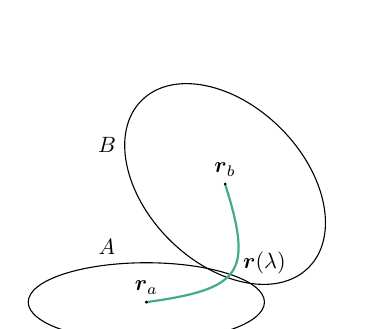
\begin{tikzpicture}

\pgfmathsetmacro{\as}{1.5};
\pgfmathsetmacro{\bs}{0.5};
\pgfmathsetmacro{\cs}{sqrt(\as^2 - \bs^2)}
\pgfmathsetmacro{\al}{1.5};
\pgfmathsetmacro{\bl}{1};
\pgfmathsetmacro{\cl}{sqrt(\al^2 - \bl^2)}
\pgfmathsetmacro{\xs}{abs(\cs - \cl)}


\draw (0, 0) ellipse [x radius = \as cm, y radius = \bs cm] node[above, scale=0.8] {$\vec{r}_a$};
\draw [rotate around={-45:(1, 1.5)}] (1,1.5) ellipse [x radius = \al cm, y radius = \bl cm] node[above, scale=0.8] {$\vec{r}_b$};

\begin{axis}[
    anchor=origin,
    x=1cm, y=1cm,
    no marks,
    clip=false,
    axis line style={draw=none},
    tick style={draw=none},
    yticklabels={,,},
    xticklabels={,,},
    ]
    % this parametric plot was calculated with mathematica
    \addplot [domain=0:1,samples=100,mygreen,thick]({(33.75*(1 - x)*x)/(9 + 47*x - 20*x^2) + ( 9*(1 - x) * (1 + (11*x)/2))/(9 + 47*x - 20*x^2)}, {5*(1 - x)*x/(2 * (9 + 47*x - 20*x^2)) + ( 1.5*(1 - x) * (9 * (1 - x) + 13 *x /2))/(9 + 47*x- 20*x^2});

\end{axis}

\node[scale=0.8] at (1.5,0.5) {$\vec{r}(\lambda )$};

\filldraw[black] (0, 0) circle [radius = 0.01 cm];
\filldraw[black] (1, 1.5) circle [radius = 0.01 cm];

\node[scale=0.8] at (-0.5,0.7) {$A$};
\node[scale=0.8] at (-0.5,2) {$B$};

\end{tikzpicture}
% 33.75*(1 - x)*x/(9 + 47*x - 20*x^2) + ( 9*(1 - x) * (1 + (11*x)/2))/(9 + 47*x - 20*x^2)
% 5*(1 - x)*x/(2 * (9 + 47*x - 20*x^2)) + ( 1.5*(1 - x) * (9 * (1 - x) + 13 *x /2))/(9 + 47*x- 20*x^2)}
    \caption{Minimalna pot $\vec{r}(\lambda)$ gre skozi presek elips $A$ in $B$.}
    \label{fig:path}
\end{figure}\\
\noindent Poglejmo kako se obnaša pot $\vec{r}(\lambda), \, \lambda \in [0,1]$, ki povezuje 
centra elips med seboj -- kar lahko vidimo na sliki~\ref{fig:path}.
Iz enačbe~\ref{eq:elipsa} sledi, da je vrednost $F(\vec{r}, \lambda)$ na območju 
izven obeh elips $F(\vec{r}, \lambda)>1$. Če se $A$ in $B$ ne sekata, potem mora imeti 
pot minimuma $F(\vec{r}, \lambda)>1$ vrednost večjo od $1$. Če se $A$ in $B$ prekrivata 
potem je vrednost $F(\vec{r}, \lambda)<1$ na preseku $A \cap B$ za katerokoli vrednost 
$\lambda \in [0,1]$.  Sledi, da je vrednost minimuma $F(\vec{r}, \lambda)<1$ zagotovo 
manjša od $1$. To pomeni, da pot $\vec{r}(\lambda)$ zagotovo ne bo šla izven območij
$A$ in $B$. Zaključimo, da za vrednosti $F(\vec{r}(\lambda), \lambda) = 
f(\lambda)$ velja
\begin{equation}
    \max_{0<\lambda<1} f(\lambda)
    \begin{cases}
        <1 \quad\text{$A$ in $B$ se prekrivata,}\\
        =1 \quad\text{$A$ in $B$ sta tangentni,}\\
        >1 \quad\text{$A$ in $B$ se ne dotikata.}
    \end{cases}
    \label{eq:kriterij}
\end{equation}
Te lastnosti izkoristimo pri definiciji kontaktne funkcije med dvema elipsama, tako da
velja
\begin{equation}
    F_{A B}(\vec{r}_{A B}, \theta_A, \theta_B) =
    \max_{0<\lambda<1} f(\lambda) = \mu^2.
    \label{eq:kontakt}
\end{equation}
Vrednost $\mu$ je linearni faktor s~katerim moramo množiti elipsi $A$ in $B$, da 
postaneta tangentni.
\subsection{Zaznavanje prekrivanj s~kontaktno funkcijo}
Vpeljano kontaktno funkcijo uporabimo na porazdelitvi elips, ki smo jo zgenerirali
z~Mitchellovim algoritmom. 
Za primer poglejmo sliko~\ref{fig:zaznavanje_trkov}, ki prikazuje porazdelitev
$128$ elips. Izberemo naključno elipso in pogledamo njeno okolico polmera $2a$.
S~tem zmanjšamo število parov elips na katerih moramo računati kontaktno funkcijo.
\begin{figure}[!ht]
    \centering
    \resizebox{.32\textwidth}{!}{% This file was created with tikzplotlib v0.10.1.
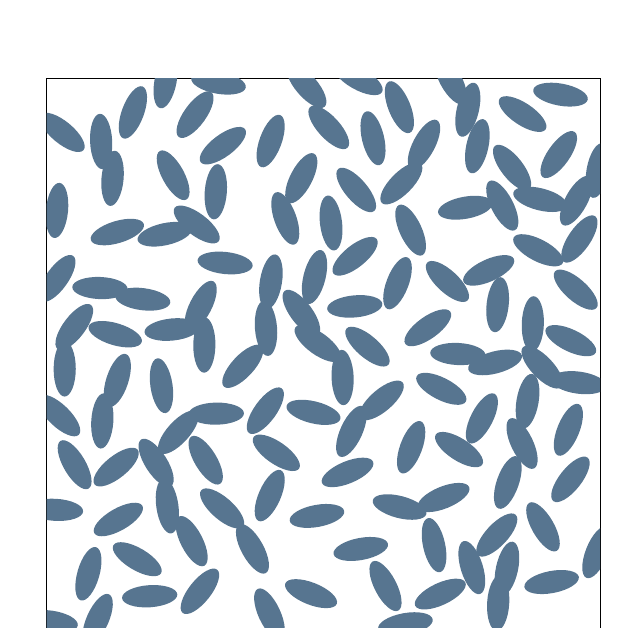
\begin{tikzpicture}

\definecolor{darkgray176}{RGB}{176,176,176}
\definecolor{steelblue31119180}{RGB}{31,119,180}

\begin{axis}[
    x=2, y=2,
    x grid style={darkgray176},
    xmin=0, xmax=100,
    y grid style={darkgray176},
    ymin=0, ymax=100,
    tick style={draw=none},
    yticklabels={,,},
    xtick
]
\draw[draw=none,fill=myblue,rotate around={260.204650150668:(axis cs:86.882913846962,41.6777189680256)}] (axis cs:86.882913846962,41.6777189680256) ellipse (5 and 2);
\draw[draw=none,fill=myblue,rotate around={352.916970683532:(axis cs:17.3702053810315,60.1099457262999)}] (axis cs:17.3702053810315,60.1099457262999) ellipse (5 and 2);
\draw[draw=none,fill=myblue,rotate around={22.6137910135262:(axis cs:54.3578505168292,28.8121800265779)}] (axis cs:54.3578505168292,28.8121800265779) ellipse (5 and 2);
\draw[draw=none,fill=myblue,rotate around={54.1605172415885:(axis cs:26.8061313592254,93.4547820902352)}] (axis cs:26.8061313592254,93.4547820902352) ellipse (5 and 2);
\draw[draw=none,fill=myblue,rotate around={349.787045848476:(axis cs:92.8377033572501,97.06536507931)}] (axis cs:92.8377033572501,97.06536507931) ellipse (5 and 2);
\draw[draw=none,fill=myblue,rotate around={301.169459612978:(axis cs:28.7329585023873,31.0188006699616)}] (axis cs:28.7329585023873,31.0188006699616) ellipse (5 and 2);
\draw[draw=none,fill=myblue,rotate around={9.99665572168897:(axis cs:64.8146228143106,1.40202864166694)}] (axis cs:64.8146228143106,1.40202864166694) ellipse (5 and 2);
\draw[draw=none,fill=myblue,rotate around={75.9590718992238:(axis cs:48.3915146177629,64.1181420805372)}] (axis cs:48.3915146177629,64.1181420805372) ellipse (5 and 2);
\draw[draw=none,fill=myblue,rotate around={227.038747519095:(axis cs:81.3272540913949,17.500793155944)}] (axis cs:81.3272540913949,17.500793155944) ellipse (5 and 2);
\draw[draw=none,fill=myblue,rotate around={248.168331406681:(axis cs:99.3939573851162,14.3982292725168)}] (axis cs:99.3939573851162,14.3982292725168) ellipse (5 and 2);
\draw[draw=none,fill=myblue,rotate around={190.315288515932:(axis cs:75.6429101109758,76.6325837014612)}] (axis cs:75.6429101109758,76.6325837014612) ellipse (5 and 2);
\draw[draw=none,fill=myblue,rotate around={52.992867030674:(axis cs:4.98633355030644,55.0858130674453)}] (axis cs:4.98633355030644,55.0858130674453) ellipse (5 and 2);
\draw[draw=none,fill=myblue,rotate around={54.0037365377994:(axis cs:39.5055460595019,39.9625444177252)}] (axis cs:39.5055460595019,39.9625444177252) ellipse (5 and 2);
\draw[draw=none,fill=myblue,rotate around={332.863827568311:(axis cs:71.3013949179524,43.9153887693566)}] (axis cs:71.3013949179524,43.9153887693566) ellipse (5 and 2);
\draw[draw=none,fill=myblue,rotate around={84.5473125880316:(axis cs:1.86286810442203,76.1448652422809)}] (axis cs:1.86286810442203,76.1448652422809) ellipse (5 and 2);
\draw[draw=none,fill=myblue,rotate around={294.754598975761:(axis cs:40.2510821396431,3.23948125486693)}] (axis cs:40.2510821396431,3.23948125486693) ellipse (5 and 2);
\draw[draw=none,fill=myblue,rotate around={353.860974913289:(axis cs:32.2412530863386,66.6502536503754)}] (axis cs:32.2412530863386,66.6502536503754) ellipse (5 and 2);
\draw[draw=none,fill=myblue,rotate around={268.079369117024:(axis cs:87.8331224981219,55.6504236167273)}] (axis cs:87.8331224981219,55.6504236167273) ellipse (5 and 2);
\draw[draw=none,fill=myblue,rotate around={249.914628955572:(axis cs:40.4644776697715,88.6819898491135)}] (axis cs:40.4644776697715,88.6819898491135) ellipse (5 and 2);
\draw[draw=none,fill=myblue,rotate around={315.9419617351:(axis cs:2.21483365114915,39.0946442609324)}] (axis cs:2.21483365114915,39.0946442609324) ellipse (5 and 2);
\draw[draw=none,fill=myblue,rotate around={29.7482081236702:(axis cs:12.948532403687,20.3052301632043)}] (axis cs:12.948532403687,20.3052301632043) ellipse (5 and 2);
\draw[draw=none,fill=myblue,rotate around={245.9296477557:(axis cs:9.21255957094804,2.22727254610813)}] (axis cs:9.21255957094804,2.22727254610813) ellipse (5 and 2);
\draw[draw=none,fill=myblue,rotate around={10.5803347867585:(axis cs:56.7525384036258,14.9822704642782)}] (axis cs:56.7525384036258,14.9822704642782) ellipse (5 and 2);
\draw[draw=none,fill=myblue,rotate around={231.67969665037:(axis cs:94.6296514046673,27.5593228059429)}] (axis cs:94.6296514046673,27.5593228059429) ellipse (5 and 2);
\draw[draw=none,fill=myblue,rotate around={246.320529683567:(axis cs:40.2988588854947,24.6222243618935)}] (axis cs:40.2988588854947,24.6222243618935) ellipse (5 and 2);
\draw[draw=none,fill=myblue,rotate around={345.812285412304:(axis cs:89.1671087210519,78.1531769002003)}] (axis cs:89.1671087210519,78.1531769002003) ellipse (5 and 2);
\draw[draw=none,fill=myblue,rotate around={319.270432431842:(axis cs:57.9576260069661,51.5378189312098)}] (axis cs:57.9576260069661,51.5378189312098) ellipse (5 and 2);
\draw[draw=none,fill=myblue,rotate around={98.5717374651543:(axis cs:20.7427655078686,44.4798361153012)}] (axis cs:20.7427655078686,44.4798361153012) ellipse (5 and 2);
\draw[draw=none,fill=myblue,rotate around={320.301578164404:(axis cs:2.81441707119023,90.2466579598913)}] (axis cs:2.81441707119023,90.2466579598913) ellipse (5 and 2);
\draw[draw=none,fill=myblue,rotate around={76.4647671337003:(axis cs:76.0905857450005,94.3357690743821)}] (axis cs:76.0905857450005,94.3357690743821) ellipse (5 and 2);
\draw[draw=none,fill=myblue,rotate around={84.9272953979372:(axis cs:11.9019594584809,81.9433638347379)}] (axis cs:11.9019594584809,81.9433638347379) ellipse (5 and 2);
\draw[draw=none,fill=myblue,rotate around={204.607367274743:(axis cs:79.8625822264079,65.311187764344)}] (axis cs:79.8625822264079,65.311187764344) ellipse (5 and 2);
\draw[draw=none,fill=myblue,rotate around={12.3739793687086:(axis cs:21.323586325317,71.8427228400097)}] (axis cs:21.323586325317,71.8427228400097) ellipse (5 and 2);
\draw[draw=none,fill=myblue,rotate around={117.168001814191:(axis cs:26.195767740668,16.3937377096593)}] (axis cs:26.195767740668,16.3937377096593) ellipse (5 and 2);
\draw[draw=none,fill=myblue,rotate around={274.460391494636:(axis cs:39.6281320324819,54.8484672789167)}] (axis cs:39.6281320324819,54.8484672789167) ellipse (5 and 2);
\draw[draw=none,fill=myblue,rotate around={130.54913502052:(axis cs:55.933435835093,79.8429238370018)}] (axis cs:55.933435835093,79.8429238370018) ellipse (5 and 2);
\draw[draw=none,fill=myblue,rotate around={132.433882308199:(axis cs:50.9653840442826,91.1428552378015)}] (axis cs:50.9653840442826,91.1428552378015) ellipse (5 and 2);
\draw[draw=none,fill=myblue,rotate around={69.0335688009109:(axis cs:63.3896028126425,63.0007610550364)}] (axis cs:63.3896028126425,63.0007610550364) ellipse (5 and 2);
\draw[draw=none,fill=myblue,rotate around={3.85375435108094:(axis cs:18.6121409896952,6.44416862770173)}] (axis cs:18.6121409896952,6.44416862770173) ellipse (5 and 2);
\draw[draw=none,fill=myblue,rotate around={242.14725970489:(axis cs:68.1720522704402,88.0252489706398)}] (axis cs:68.1720522704402,88.0252489706398) ellipse (5 and 2);
\draw[draw=none,fill=myblue,rotate around={289.801943190306:(axis cs:43.1108191914449,74.7060050602938)}] (axis cs:43.1108191914449,74.7060050602938) ellipse (5 and 2);
\draw[draw=none,fill=myblue,rotate around={282.464320644406:(axis cs:69.9923435700512,15.6729689301564)}] (axis cs:69.9923435700512,15.6729689301564) ellipse (5 and 2);
\draw[draw=none,fill=myblue,rotate around={234.724822456551:(axis cs:1.89041207297357,63.8556494308399)}] (axis cs:1.89041207297357,63.8556494308399) ellipse (5 and 2);
\draw[draw=none,fill=myblue,rotate around={302.616093260557:(axis cs:19.772606026042,30.5471205146096)}] (axis cs:19.772606026042,30.5471205146096) ellipse (5 and 2);
\draw[draw=none,fill=myblue,rotate around={158.340760048643:(axis cs:47.7631607343279,6.91010886104096)}] (axis cs:47.7631607343279,6.91010886104096) ellipse (5 and 2);
\draw[draw=none,fill=myblue,rotate around={202.054523659658:(axis cs:71.7026363458189,24.2772963730362)}] (axis cs:71.7026363458189,24.2772963730362) ellipse (5 and 2);
\draw[draw=none,fill=myblue,rotate around={69.6380570029668:(axis cs:15.5768836156765,93.8502782854917)}] (axis cs:15.5768836156765,93.8502782854917) ellipse (5 and 2);
\draw[draw=none,fill=myblue,rotate around={152.575999415476:(axis cs:88.8183765619847,68.9473725156417)}] (axis cs:88.8183765619847,68.9473725156417) ellipse (5 and 2);
\draw[draw=none,fill=myblue,rotate around={86.6229821231618:(axis cs:81.5765245617972,5.2010753658165)}] (axis cs:81.5765245617972,5.2010753658165) ellipse (5 and 2);
\draw[draw=none,fill=myblue,rotate around={69.5870529278177:(axis cs:65.8506228342984,33.3603805241784)}] (axis cs:65.8506228342984,33.3603805241784) ellipse (5 and 2);
\draw[draw=none,fill=myblue,rotate around={89.4563598649543:(axis cs:28.4867819268627,51.8325293958749)}] (axis cs:28.4867819268627,51.8325293958749) ellipse (5 and 2);
\draw[draw=none,fill=myblue,rotate around={118.92867917955:(axis cs:37.1783840900199,15.0048162820745)}] (axis cs:37.1783840900199,15.0048162820745) ellipse (5 and 2);
\draw[draw=none,fill=myblue,rotate around={10.7885285332415:(axis cs:91.2306043988741,9.00705471851809)}] (axis cs:91.2306043988741,9.00705471851809) ellipse (5 and 2);
\draw[draw=none,fill=myblue,rotate around={70.766031758227:(axis cs:83.3116224870324,26.9941651840805)}] (axis cs:83.3116224870324,26.9941651840805) ellipse (5 and 2);
\draw[draw=none,fill=myblue,rotate around={35.6434088614135:(axis cs:68.8597459043663,54.9424041219192)}] (axis cs:68.8597459043663,54.9424041219192) ellipse (5 and 2);
\draw[draw=none,fill=myblue,rotate around={51.5476613473339:(axis cs:27.6855305634842,7.33028459895518)}] (axis cs:27.6855305634842,7.33028459895518) ellipse (5 and 2);
\draw[draw=none,fill=myblue,rotate around={346.299933178858:(axis cs:48.2056048404719,39.6634016751004)}] (axis cs:48.2056048404719,39.6634016751004) ellipse (5 and 2);
\draw[draw=none,fill=myblue,rotate around={265.618518135428:(axis cs:30.5569873761105,79.5161765830348)}] (axis cs:30.5569873761105,79.5161765830348) ellipse (5 and 2);
\draw[draw=none,fill=myblue,rotate around={103.45201055566:(axis cs:58.9588736685684,89.1863749433072)}] (axis cs:58.9588736685684,89.1863749433072) ellipse (5 and 2);
\draw[draw=none,fill=myblue,rotate around={220.502650942834:(axis cs:60.5080407877913,41.8210802578143)}] (axis cs:60.5080407877913,41.8210802578143) ellipse (5 and 2);
\draw[draw=none,fill=myblue,rotate around={218.80828811829:(axis cs:55.7205303388384,67.860496152752)}] (axis cs:55.7205303388384,67.860496152752) ellipse (5 and 2);
\draw[draw=none,fill=myblue,rotate around={150.520494903969:(axis cs:56.2460532738079,99.98891155317)}] (axis cs:56.2460532738079,99.98891155317) ellipse (5 and 2);
\draw[draw=none,fill=myblue,rotate around={54.8255110517293:(axis cs:92.5194453046932,86.236230748634)}] (axis cs:92.5194453046932,86.236230748634) ellipse (5 and 2);
\draw[draw=none,fill=myblue,rotate around={300.366524500867:(axis cs:5.04996349555212,30.2011265445795)}] (axis cs:5.04996349555212,30.2011265445795) ellipse (5 and 2);
\draw[draw=none,fill=myblue,rotate around={254.060351773917:(axis cs:7.53779290855019,10.5024775779718)}] (axis cs:7.53779290855019,10.5024775779718) ellipse (5 and 2);
\draw[draw=none,fill=myblue,rotate around={294.878692522367:(axis cs:65.7557552355382,72.5896944885608)}] (axis cs:65.7557552355382,72.5896944885608) ellipse (5 and 2);
\draw[draw=none,fill=myblue,rotate around={16.7930611338574:(axis cs:12.7640613253374,72.239375523327)}] (axis cs:12.7640613253374,72.239375523327) ellipse (5 and 2);
\draw[draw=none,fill=myblue,rotate around={86.396868066909:(axis cs:10.0538312195155,38.1153271806579)}] (axis cs:10.0538312195155,38.1153271806579) ellipse (5 and 2);
\draw[draw=none,fill=myblue,rotate around={324.027291154328:(axis cs:49.0019491046676,52.1085809997291)}] (axis cs:49.0019491046676,52.1085809997291) ellipse (5 and 2);
\draw[draw=none,fill=myblue,rotate around={67.9654909980869:(axis cs:94.255974386524,36.5108506935766)}] (axis cs:94.255974386524,36.5108506935766) ellipse (5 and 2);
\draw[draw=none,fill=myblue,rotate around={251.941321158686:(axis cs:12.763648487112,45.4459238854269)}] (axis cs:12.763648487112,45.4459238854269) ellipse (5 and 2);
\draw[draw=none,fill=myblue,rotate around={190.351190759998:(axis cs:48.833234251249,20.9506374190798)}] (axis cs:48.833234251249,20.9506374190798) ellipse (5 and 2);
\draw[draw=none,fill=myblue,rotate around={298.612113224356:(axis cs:22.8495523863503,82.5045499767124)}] (axis cs:22.8495523863503,82.5045499767124) ellipse (5 and 2);
\draw[draw=none,fill=myblue,rotate around={352.400434801704:(axis cs:96.1055748110164,45.0288993232664)}] (axis cs:96.1055748110164,45.0288993232664) ellipse (5 and 2);
\draw[draw=none,fill=myblue,rotate around={24.9758141740133:(axis cs:71.1141108281389,6.83262257865851)}] (axis cs:71.1141108281389,6.83262257865851) ellipse (5 and 2);
\draw[draw=none,fill=myblue,rotate around={47.1120904509369:(axis cs:35.4257600506402,47.9798120950139)}] (axis cs:35.4257600506402,47.9798120950139) ellipse (5 and 2);
\draw[draw=none,fill=myblue,rotate around={14.7746567560795:(axis cs:81.0140107259634,48.6829084944324)}] (axis cs:81.0140107259634,48.6829084944324) ellipse (5 and 2);
\draw[draw=none,fill=myblue,rotate around={307.896545207601:(axis cs:84.0823937105312,83.8764630495301)}] (axis cs:84.0823937105312,83.8764630495301) ellipse (5 and 2);
\draw[draw=none,fill=myblue,rotate around={185.319571851166:(axis cs:55.6619378201471,58.8078579678459)}] (axis cs:55.6619378201471,58.8078579678459) ellipse (5 and 2);
\draw[draw=none,fill=myblue,rotate around={325.172336062301:(axis cs:41.4907403776405,32.3506445488188)}] (axis cs:41.4907403776405,32.3506445488188) ellipse (5 and 2);
\draw[draw=none,fill=myblue,rotate around={119.872128201725:(axis cs:89.6719005334523,18.9791507390857)}] (axis cs:89.6719005334523,18.9791507390857) ellipse (5 and 2);
\draw[draw=none,fill=myblue,rotate around={357.821530747641:(axis cs:9.62782038925507,62.1232922938803)}] (axis cs:9.62782038925507,62.1232922938803) ellipse (5 and 2);
\draw[draw=none,fill=myblue,rotate around={326.408690547729:(axis cs:85.9872570382636,93.5585714150404)}] (axis cs:85.9872570382636,93.5585714150404) ellipse (5 and 2);
\draw[draw=none,fill=myblue,rotate around={165.491621211313:(axis cs:63.768546413739,22.5593396318724)}] (axis cs:63.768546413739,22.5593396318724) ellipse (5 and 2);
\draw[draw=none,fill=myblue,rotate around={62.5689723853916:(axis cs:45.999869632787,81.9718303639362)}] (axis cs:45.999869632787,81.9718303639362) ellipse (5 and 2);
\draw[draw=none,fill=myblue,rotate around={80.686868301937:(axis cs:40.513972119891,63.2574647102097)}] (axis cs:40.513972119891,63.2574647102097) ellipse (5 and 2);
\draw[draw=none,fill=myblue,rotate around={352.160175168487:(axis cs:0.670179449571862,1.8587023245636)}] (axis cs:0.670179449571862,1.8587023245636) ellipse (5 and 2);
\draw[draw=none,fill=myblue,rotate around={147.152087004351:(axis cs:74.5059127687272,32.94117457168)}] (axis cs:74.5059127687272,32.94117457168) ellipse (5 and 2);
\draw[draw=none,fill=myblue,rotate around={79.912177589682:(axis cs:99.5409900854364,83.3507452903862)}] (axis cs:99.5409900854364,83.3507452903862) ellipse (5 and 2);
\draw[draw=none,fill=myblue,rotate around={0.893218153011031:(axis cs:30.6413648667477,39.4308194959482)}] (axis cs:30.6413648667477,39.4308194959482) ellipse (5 and 2);
\draw[draw=none,fill=myblue,rotate around={149.39430802483:(axis cs:16.364079445829,13.1332597438818)}] (axis cs:16.364079445829,13.1332597438818) ellipse (5 and 2);
\draw[draw=none,fill=myblue,rotate around={263.614140785283:(axis cs:81.4779667377777,59.1129447486611)}] (axis cs:81.4779667377777,59.1129447486611) ellipse (5 and 2);
\draw[draw=none,fill=myblue,rotate around={356.776002302174:(axis cs:1.58847438749508,22.0501701614518)}] (axis cs:1.58847438749508,22.0501701614518) ellipse (5 and 2);
\draw[draw=none,fill=myblue,rotate around={170.091144245238:(axis cs:31.0423654417477,99.2149038897966)}] (axis cs:31.0423654417477,99.2149038897966) ellipse (5 and 2);
\draw[draw=none,fill=myblue,rotate around={130.754835632223:(axis cs:46.9468771825903,98.6594198824206)}] (axis cs:46.9468771825903,98.6594198824206) ellipse (5 and 2);
\draw[draw=none,fill=myblue,rotate around={177.160830537073:(axis cs:74.2938016624452,50.2051842249504)}] (axis cs:74.2938016624452,50.2051842249504) ellipse (5 and 2);
\draw[draw=none,fill=myblue,rotate around={242.728282134562:(axis cs:78.6279318778352,38.5714724755397)}] (axis cs:78.6279318778352,38.5714724755397) ellipse (5 and 2);
\draw[draw=none,fill=myblue,rotate around={92.6718119634767:(axis cs:9.83995614919241,88.6061914819749)}] (axis cs:9.83995614919241,88.6061914819749) ellipse (5 and 2);
\draw[draw=none,fill=myblue,rotate around={154.348461856241:(axis cs:94.6984370754419,52.6195822773216)}] (axis cs:94.6984370754419,52.6195822773216) ellipse (5 and 2);
\draw[draw=none,fill=myblue,rotate around={163.428804825857:(axis cs:12.3813878424189,53.7827644674075)}] (axis cs:12.3813878424189,53.7827644674075) ellipse (5 and 2);
\draw[draw=none,fill=myblue,rotate around={242.708068430962:(axis cs:27.8300822695283,58.8917633929874)}] (axis cs:27.8300822695283,58.8917633929874) ellipse (5 and 2);
\draw[draw=none,fill=myblue,rotate around={235.475628484884:(axis cs:96.2473706632951,70.984470876944)}] (axis cs:96.2473706632951,70.984470876944) ellipse (5 and 2);
\draw[draw=none,fill=myblue,rotate around={36.656268675175:(axis cs:31.8306870443883,87.8458564448473)}] (axis cs:31.8306870443883,87.8458564448473) ellipse (5 and 2);
\draw[draw=none,fill=myblue,rotate around={112.043249573373:(axis cs:63.7252837899546,94.8004298199742)}] (axis cs:63.7252837899546,94.8004298199742) ellipse (5 and 2);
\draw[draw=none,fill=myblue,rotate around={92.0523885815362:(axis cs:53.4661151748034,45.9549267427767)}] (axis cs:53.4661151748034,45.9549267427767) ellipse (5 and 2);
\draw[draw=none,fill=myblue,rotate around={245.449379453127:(axis cs:55.0511046066284,36.2202640673709)}] (axis cs:55.0511046066284,36.2202640673709) ellipse (5 and 2);
\draw[draw=none,fill=myblue,rotate around={295.652389779659:(axis cs:85.8883818155678,34.0384614709201)}] (axis cs:85.8883818155678,34.0384614709201) ellipse (5 and 2);
\draw[draw=none,fill=myblue,rotate around={225.194198562187:(axis cs:64.0823849056176,81.0403814957276)}] (axis cs:64.0823849056176,81.0403814957276) ellipse (5 and 2);
\draw[draw=none,fill=myblue,rotate around={96.995820274412:(axis cs:51.3744048894096,73.8743045476509)}] (axis cs:51.3744048894096,73.8743045476509) ellipse (5 and 2);
\draw[draw=none,fill=myblue,rotate around={98.0898695872326:(axis cs:21.8022369733386,22.7350748099463)}] (axis cs:21.8022369733386,22.7350748099463) ellipse (5 and 2);
\draw[draw=none,fill=myblue,rotate around={138.78854758218:(axis cs:31.6959886698282,22.3058845988067)}] (axis cs:31.6959886698282,22.3058845988067) ellipse (5 and 2);
\draw[draw=none,fill=myblue,rotate around={318.492823597775:(axis cs:95.5877271140043,61.8264497134761)}] (axis cs:95.5877271140043,61.8264497134761) ellipse (5 and 2);
\draw[draw=none,fill=myblue,rotate around={259.231220358722:(axis cs:21.4771599692152,99.5192993241954)}] (axis cs:21.4771599692152,99.5192993241954) ellipse (5 and 2);
\draw[draw=none,fill=myblue,rotate around={269.741531872192:(axis cs:3.25648736233763,47.5197410511917)}] (axis cs:3.25648736233763,47.5197410511917) ellipse (5 and 2);
\draw[draw=none,fill=myblue,rotate around={297.353285854387:(axis cs:61.218038462067,8.28676729492537)}] (axis cs:61.218038462067,8.28676729492537) ellipse (5 and 2);
\draw[draw=none,fill=myblue,rotate around={47.726999713751:(axis cs:23.780568342442,36.0723097613012)}] (axis cs:23.780568342442,36.0723097613012) ellipse (5 and 2);
\draw[draw=none,fill=myblue,rotate around={77.7238081358585:(axis cs:83.1646923435251,11.4032470035099)}] (axis cs:83.1646923435251,11.4032470035099) ellipse (5 and 2);
\draw[draw=none,fill=myblue,rotate around={317.080766857636:(axis cs:72.4044215935182,63.3080070150894)}] (axis cs:72.4044215935182,63.3080070150894) ellipse (5 and 2);
\draw[draw=none,fill=myblue,rotate around={38.7891838094475:(axis cs:12.5489499377054,29.7759902549972)}] (axis cs:12.5489499377054,29.7759902549972) ellipse (5 and 2);
\draw[draw=none,fill=myblue,rotate around={313.711203512664:(axis cs:89.5227528142594,47.8325968256834)}] (axis cs:89.5227528142594,47.8325968256834) ellipse (5 and 2);
\draw[draw=none,fill=myblue,rotate around={298.477328346312:(axis cs:72.9707250021413,99.7706074619335)}] (axis cs:72.9707250021413,99.7706074619335) ellipse (5 and 2);
\draw[draw=none,fill=myblue,rotate around={5.81423179660655:(axis cs:22.6543381808917,54.6284359265346)}] (axis cs:22.6543381808917,54.6284359265346) ellipse (5 and 2);
\draw[draw=none,fill=myblue,rotate around={107.369343119315:(axis cs:76.8084025367909,11.622625330049)}] (axis cs:76.8084025367909,11.622625330049) ellipse (5 and 2);
\draw[draw=none,fill=myblue,rotate around={297.410687409085:(axis cs:82.316163382063,77.0255989351747)}] (axis cs:82.316163382063,77.0255989351747) ellipse (5 and 2);
\draw[draw=none,fill=myblue,rotate around={241.412768220482:(axis cs:95.6908177165746,77.8990008145085)}] (axis cs:95.6908177165746,77.8990008145085) ellipse (5 and 2);
\draw[draw=none,fill=myblue,rotate around={306.721684207499:(axis cs:46.0121623420069,57.6240632220017)}] (axis cs:46.0121623420069,57.6240632220017) ellipse (5 and 2);
\draw[draw=none,fill=myblue,rotate around={322.736476985811:(axis cs:27.1112894933776,73.6073827622796)}] (axis cs:27.1112894933776,73.6073827622796) ellipse (5 and 2);
\draw[draw=none,fill=myblue,rotate around={77.4649729853431:(axis cs:77.8123782915191,87.7467385017039)}] (axis cs:77.8123782915191,87.7467385017039) ellipse (5 and 2);
\end{axis}

\end{tikzpicture}
}
    \resizebox{.32\textwidth}{!}{% This file was created with tikzplotlib v0.10.1.
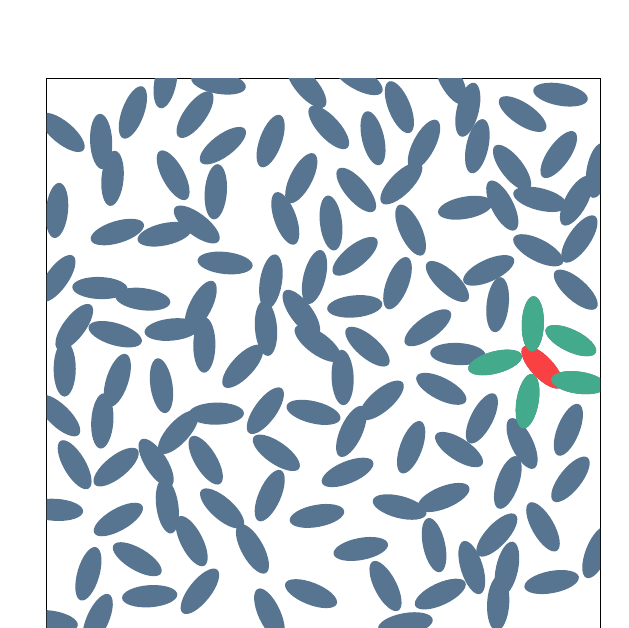
\begin{tikzpicture}

\definecolor{darkgray176}{RGB}{176,176,176}
\definecolor{gray}{RGB}{128,128,128}
\definecolor{steelblue31119180}{RGB}{31,119,180}

\begin{axis}[
    x=2, y=2,
    x grid style={darkgray176},
    xmin=0, xmax=100,
    y grid style={darkgray176},
    ymin=0, ymax=100,
    tick style={draw=none},
    yticklabels={,,},
    xtick
]
\draw[draw=none,fill=myblue,rotate around={260.204650150668:(axis cs:86.882913846962,41.6777189680256)}] (axis cs:86.882913846962,41.6777189680256) ellipse (5 and 2);
\draw[draw=none,fill=myblue,rotate around={352.916970683532:(axis cs:17.3702053810315,60.1099457262999)}] (axis cs:17.3702053810315,60.1099457262999) ellipse (5 and 2);
\draw[draw=none,fill=myblue,rotate around={22.6137910135262:(axis cs:54.3578505168292,28.8121800265779)}] (axis cs:54.3578505168292,28.8121800265779) ellipse (5 and 2);
\draw[draw=none,fill=myblue,rotate around={54.1605172415885:(axis cs:26.8061313592254,93.4547820902352)}] (axis cs:26.8061313592254,93.4547820902352) ellipse (5 and 2);
\draw[draw=none,fill=myblue,rotate around={349.787045848476:(axis cs:92.8377033572501,97.06536507931)}] (axis cs:92.8377033572501,97.06536507931) ellipse (5 and 2);
\draw[draw=none,fill=myblue,rotate around={301.169459612978:(axis cs:28.7329585023873,31.0188006699616)}] (axis cs:28.7329585023873,31.0188006699616) ellipse (5 and 2);
\draw[draw=none,fill=myblue,rotate around={9.99665572168897:(axis cs:64.8146228143106,1.40202864166694)}] (axis cs:64.8146228143106,1.40202864166694) ellipse (5 and 2);
\draw[draw=none,fill=myblue,rotate around={75.9590718992238:(axis cs:48.3915146177629,64.1181420805372)}] (axis cs:48.3915146177629,64.1181420805372) ellipse (5 and 2);
\draw[draw=none,fill=myblue,rotate around={227.038747519095:(axis cs:81.3272540913949,17.500793155944)}] (axis cs:81.3272540913949,17.500793155944) ellipse (5 and 2);
\draw[draw=none,fill=myblue,rotate around={248.168331406681:(axis cs:99.3939573851162,14.3982292725168)}] (axis cs:99.3939573851162,14.3982292725168) ellipse (5 and 2);
\draw[draw=none,fill=myblue,rotate around={190.315288515932:(axis cs:75.6429101109758,76.6325837014612)}] (axis cs:75.6429101109758,76.6325837014612) ellipse (5 and 2);
\draw[draw=none,fill=myblue,rotate around={52.992867030674:(axis cs:4.98633355030644,55.0858130674453)}] (axis cs:4.98633355030644,55.0858130674453) ellipse (5 and 2);
\draw[draw=none,fill=myblue,rotate around={54.0037365377994:(axis cs:39.5055460595019,39.9625444177252)}] (axis cs:39.5055460595019,39.9625444177252) ellipse (5 and 2);
\draw[draw=none,fill=myblue,rotate around={332.863827568311:(axis cs:71.3013949179524,43.9153887693566)}] (axis cs:71.3013949179524,43.9153887693566) ellipse (5 and 2);
\draw[draw=none,fill=myblue,rotate around={84.5473125880316:(axis cs:1.86286810442203,76.1448652422809)}] (axis cs:1.86286810442203,76.1448652422809) ellipse (5 and 2);
\draw[draw=none,fill=myblue,rotate around={294.754598975761:(axis cs:40.2510821396431,3.23948125486693)}] (axis cs:40.2510821396431,3.23948125486693) ellipse (5 and 2);
\draw[draw=none,fill=myblue,rotate around={353.860974913289:(axis cs:32.2412530863386,66.6502536503754)}] (axis cs:32.2412530863386,66.6502536503754) ellipse (5 and 2);
\draw[draw=none,fill=myblue,rotate around={268.079369117024:(axis cs:87.8331224981219,55.6504236167273)}] (axis cs:87.8331224981219,55.6504236167273) ellipse (5 and 2);
\draw[draw=none,fill=myblue,rotate around={249.914628955572:(axis cs:40.4644776697715,88.6819898491135)}] (axis cs:40.4644776697715,88.6819898491135) ellipse (5 and 2);
\draw[draw=none,fill=myblue,rotate around={315.9419617351:(axis cs:2.21483365114915,39.0946442609324)}] (axis cs:2.21483365114915,39.0946442609324) ellipse (5 and 2);
\draw[draw=none,fill=myblue,rotate around={29.7482081236702:(axis cs:12.948532403687,20.3052301632043)}] (axis cs:12.948532403687,20.3052301632043) ellipse (5 and 2);
\draw[draw=none,fill=myblue,rotate around={245.9296477557:(axis cs:9.21255957094804,2.22727254610813)}] (axis cs:9.21255957094804,2.22727254610813) ellipse (5 and 2);
\draw[draw=none,fill=myblue,rotate around={10.5803347867585:(axis cs:56.7525384036258,14.9822704642782)}] (axis cs:56.7525384036258,14.9822704642782) ellipse (5 and 2);
\draw[draw=none,fill=myblue,rotate around={231.67969665037:(axis cs:94.6296514046673,27.5593228059429)}] (axis cs:94.6296514046673,27.5593228059429) ellipse (5 and 2);
\draw[draw=none,fill=myblue,rotate around={246.320529683567:(axis cs:40.2988588854947,24.6222243618935)}] (axis cs:40.2988588854947,24.6222243618935) ellipse (5 and 2);
\draw[draw=none,fill=myblue,rotate around={345.812285412304:(axis cs:89.1671087210519,78.1531769002003)}] (axis cs:89.1671087210519,78.1531769002003) ellipse (5 and 2);
\draw[draw=none,fill=myblue,rotate around={319.270432431842:(axis cs:57.9576260069661,51.5378189312098)}] (axis cs:57.9576260069661,51.5378189312098) ellipse (5 and 2);
\draw[draw=none,fill=myblue,rotate around={98.5717374651543:(axis cs:20.7427655078686,44.4798361153012)}] (axis cs:20.7427655078686,44.4798361153012) ellipse (5 and 2);
\draw[draw=none,fill=myblue,rotate around={320.301578164404:(axis cs:2.81441707119023,90.2466579598913)}] (axis cs:2.81441707119023,90.2466579598913) ellipse (5 and 2);
\draw[draw=none,fill=myblue,rotate around={76.4647671337003:(axis cs:76.0905857450005,94.3357690743821)}] (axis cs:76.0905857450005,94.3357690743821) ellipse (5 and 2);
\draw[draw=none,fill=myblue,rotate around={84.9272953979372:(axis cs:11.9019594584809,81.9433638347379)}] (axis cs:11.9019594584809,81.9433638347379) ellipse (5 and 2);
\draw[draw=none,fill=myblue,rotate around={204.607367274743:(axis cs:79.8625822264079,65.311187764344)}] (axis cs:79.8625822264079,65.311187764344) ellipse (5 and 2);
\draw[draw=none,fill=myblue,rotate around={12.3739793687086:(axis cs:21.323586325317,71.8427228400097)}] (axis cs:21.323586325317,71.8427228400097) ellipse (5 and 2);
\draw[draw=none,fill=myblue,rotate around={117.168001814191:(axis cs:26.195767740668,16.3937377096593)}] (axis cs:26.195767740668,16.3937377096593) ellipse (5 and 2);
\draw[draw=none,fill=myblue,rotate around={274.460391494636:(axis cs:39.6281320324819,54.8484672789167)}] (axis cs:39.6281320324819,54.8484672789167) ellipse (5 and 2);
\draw[draw=none,fill=myblue,rotate around={130.54913502052:(axis cs:55.933435835093,79.8429238370018)}] (axis cs:55.933435835093,79.8429238370018) ellipse (5 and 2);
\draw[draw=none,fill=myblue,rotate around={132.433882308199:(axis cs:50.9653840442826,91.1428552378015)}] (axis cs:50.9653840442826,91.1428552378015) ellipse (5 and 2);
\draw[draw=none,fill=myblue,rotate around={69.0335688009109:(axis cs:63.3896028126425,63.0007610550364)}] (axis cs:63.3896028126425,63.0007610550364) ellipse (5 and 2);
\draw[draw=none,fill=myblue,rotate around={3.85375435108094:(axis cs:18.6121409896952,6.44416862770173)}] (axis cs:18.6121409896952,6.44416862770173) ellipse (5 and 2);
\draw[draw=none,fill=myblue,rotate around={242.14725970489:(axis cs:68.1720522704402,88.0252489706398)}] (axis cs:68.1720522704402,88.0252489706398) ellipse (5 and 2);
\draw[draw=none,fill=myblue,rotate around={289.801943190306:(axis cs:43.1108191914449,74.7060050602938)}] (axis cs:43.1108191914449,74.7060050602938) ellipse (5 and 2);
\draw[draw=none,fill=myblue,rotate around={282.464320644406:(axis cs:69.9923435700512,15.6729689301564)}] (axis cs:69.9923435700512,15.6729689301564) ellipse (5 and 2);
\draw[draw=none,fill=myblue,rotate around={234.724822456551:(axis cs:1.89041207297357,63.8556494308399)}] (axis cs:1.89041207297357,63.8556494308399) ellipse (5 and 2);
\draw[draw=none,fill=myblue,rotate around={302.616093260557:(axis cs:19.772606026042,30.5471205146096)}] (axis cs:19.772606026042,30.5471205146096) ellipse (5 and 2);
\draw[draw=none,fill=myblue,rotate around={158.340760048643:(axis cs:47.7631607343279,6.91010886104096)}] (axis cs:47.7631607343279,6.91010886104096) ellipse (5 and 2);
\draw[draw=none,fill=myblue,rotate around={202.054523659658:(axis cs:71.7026363458189,24.2772963730362)}] (axis cs:71.7026363458189,24.2772963730362) ellipse (5 and 2);
\draw[draw=none,fill=myblue,rotate around={69.6380570029668:(axis cs:15.5768836156765,93.8502782854917)}] (axis cs:15.5768836156765,93.8502782854917) ellipse (5 and 2);
\draw[draw=none,fill=myblue,rotate around={152.575999415476:(axis cs:88.8183765619847,68.9473725156417)}] (axis cs:88.8183765619847,68.9473725156417) ellipse (5 and 2);
\draw[draw=none,fill=myblue,rotate around={86.6229821231618:(axis cs:81.5765245617972,5.2010753658165)}] (axis cs:81.5765245617972,5.2010753658165) ellipse (5 and 2);
\draw[draw=none,fill=myblue,rotate around={69.5870529278177:(axis cs:65.8506228342984,33.3603805241784)}] (axis cs:65.8506228342984,33.3603805241784) ellipse (5 and 2);
\draw[draw=none,fill=myblue,rotate around={89.4563598649543:(axis cs:28.4867819268627,51.8325293958749)}] (axis cs:28.4867819268627,51.8325293958749) ellipse (5 and 2);
\draw[draw=none,fill=myblue,rotate around={118.92867917955:(axis cs:37.1783840900199,15.0048162820745)}] (axis cs:37.1783840900199,15.0048162820745) ellipse (5 and 2);
\draw[draw=none,fill=myblue,rotate around={10.7885285332415:(axis cs:91.2306043988741,9.00705471851809)}] (axis cs:91.2306043988741,9.00705471851809) ellipse (5 and 2);
\draw[draw=none,fill=myblue,rotate around={70.766031758227:(axis cs:83.3116224870324,26.9941651840805)}] (axis cs:83.3116224870324,26.9941651840805) ellipse (5 and 2);
\draw[draw=none,fill=myblue,rotate around={35.6434088614135:(axis cs:68.8597459043663,54.9424041219192)}] (axis cs:68.8597459043663,54.9424041219192) ellipse (5 and 2);
\draw[draw=none,fill=myblue,rotate around={51.5476613473339:(axis cs:27.6855305634842,7.33028459895518)}] (axis cs:27.6855305634842,7.33028459895518) ellipse (5 and 2);
\draw[draw=none,fill=myblue,rotate around={346.299933178858:(axis cs:48.2056048404719,39.6634016751004)}] (axis cs:48.2056048404719,39.6634016751004) ellipse (5 and 2);
\draw[draw=none,fill=myblue,rotate around={265.618518135428:(axis cs:30.5569873761105,79.5161765830348)}] (axis cs:30.5569873761105,79.5161765830348) ellipse (5 and 2);
\draw[draw=none,fill=myblue,rotate around={103.45201055566:(axis cs:58.9588736685684,89.1863749433072)}] (axis cs:58.9588736685684,89.1863749433072) ellipse (5 and 2);
\draw[draw=none,fill=myblue,rotate around={220.502650942834:(axis cs:60.5080407877913,41.8210802578143)}] (axis cs:60.5080407877913,41.8210802578143) ellipse (5 and 2);
\draw[draw=none,fill=myblue,rotate around={218.80828811829:(axis cs:55.7205303388384,67.860496152752)}] (axis cs:55.7205303388384,67.860496152752) ellipse (5 and 2);
\draw[draw=none,fill=myblue,rotate around={150.520494903969:(axis cs:56.2460532738079,99.98891155317)}] (axis cs:56.2460532738079,99.98891155317) ellipse (5 and 2);
\draw[draw=none,fill=myblue,rotate around={54.8255110517293:(axis cs:92.5194453046932,86.236230748634)}] (axis cs:92.5194453046932,86.236230748634) ellipse (5 and 2);
\draw[draw=none,fill=myblue,rotate around={300.366524500867:(axis cs:5.04996349555212,30.2011265445795)}] (axis cs:5.04996349555212,30.2011265445795) ellipse (5 and 2);
\draw[draw=none,fill=myblue,rotate around={254.060351773917:(axis cs:7.53779290855019,10.5024775779718)}] (axis cs:7.53779290855019,10.5024775779718) ellipse (5 and 2);
\draw[draw=none,fill=myblue,rotate around={294.878692522367:(axis cs:65.7557552355382,72.5896944885608)}] (axis cs:65.7557552355382,72.5896944885608) ellipse (5 and 2);
\draw[draw=none,fill=myblue,rotate around={16.7930611338574:(axis cs:12.7640613253374,72.239375523327)}] (axis cs:12.7640613253374,72.239375523327) ellipse (5 and 2);
\draw[draw=none,fill=myblue,rotate around={86.396868066909:(axis cs:10.0538312195155,38.1153271806579)}] (axis cs:10.0538312195155,38.1153271806579) ellipse (5 and 2);
\draw[draw=none,fill=myblue,rotate around={324.027291154328:(axis cs:49.0019491046676,52.1085809997291)}] (axis cs:49.0019491046676,52.1085809997291) ellipse (5 and 2);
\draw[draw=none,fill=myblue,rotate around={67.9654909980869:(axis cs:94.255974386524,36.5108506935766)}] (axis cs:94.255974386524,36.5108506935766) ellipse (5 and 2);
\draw[draw=none,fill=myblue,rotate around={251.941321158686:(axis cs:12.763648487112,45.4459238854269)}] (axis cs:12.763648487112,45.4459238854269) ellipse (5 and 2);
\draw[draw=none,fill=myblue,rotate around={190.351190759998:(axis cs:48.833234251249,20.9506374190798)}] (axis cs:48.833234251249,20.9506374190798) ellipse (5 and 2);
\draw[draw=none,fill=myblue,rotate around={298.612113224356:(axis cs:22.8495523863503,82.5045499767124)}] (axis cs:22.8495523863503,82.5045499767124) ellipse (5 and 2);
\draw[draw=none,fill=myblue,rotate around={352.400434801704:(axis cs:96.1055748110164,45.0288993232664)}] (axis cs:96.1055748110164,45.0288993232664) ellipse (5 and 2);
\draw[draw=none,fill=myblue,rotate around={24.9758141740133:(axis cs:71.1141108281389,6.83262257865851)}] (axis cs:71.1141108281389,6.83262257865851) ellipse (5 and 2);
\draw[draw=none,fill=myblue,rotate around={47.1120904509369:(axis cs:35.4257600506402,47.9798120950139)}] (axis cs:35.4257600506402,47.9798120950139) ellipse (5 and 2);
\draw[draw=none,fill=myblue,rotate around={14.7746567560795:(axis cs:81.0140107259634,48.6829084944324)}] (axis cs:81.0140107259634,48.6829084944324) ellipse (5 and 2);
\draw[draw=none,fill=myblue,rotate around={307.896545207601:(axis cs:84.0823937105312,83.8764630495301)}] (axis cs:84.0823937105312,83.8764630495301) ellipse (5 and 2);
\draw[draw=none,fill=myblue,rotate around={185.319571851166:(axis cs:55.6619378201471,58.8078579678459)}] (axis cs:55.6619378201471,58.8078579678459) ellipse (5 and 2);
\draw[draw=none,fill=myblue,rotate around={325.172336062301:(axis cs:41.4907403776405,32.3506445488188)}] (axis cs:41.4907403776405,32.3506445488188) ellipse (5 and 2);
\draw[draw=none,fill=myblue,rotate around={119.872128201725:(axis cs:89.6719005334523,18.9791507390857)}] (axis cs:89.6719005334523,18.9791507390857) ellipse (5 and 2);
\draw[draw=none,fill=myblue,rotate around={357.821530747641:(axis cs:9.62782038925507,62.1232922938803)}] (axis cs:9.62782038925507,62.1232922938803) ellipse (5 and 2);
\draw[draw=none,fill=myblue,rotate around={326.408690547729:(axis cs:85.9872570382636,93.5585714150404)}] (axis cs:85.9872570382636,93.5585714150404) ellipse (5 and 2);
\draw[draw=none,fill=myblue,rotate around={165.491621211313:(axis cs:63.768546413739,22.5593396318724)}] (axis cs:63.768546413739,22.5593396318724) ellipse (5 and 2);
\draw[draw=none,fill=myblue,rotate around={62.5689723853916:(axis cs:45.999869632787,81.9718303639362)}] (axis cs:45.999869632787,81.9718303639362) ellipse (5 and 2);
\draw[draw=none,fill=myblue,rotate around={80.686868301937:(axis cs:40.513972119891,63.2574647102097)}] (axis cs:40.513972119891,63.2574647102097) ellipse (5 and 2);
\draw[draw=none,fill=myblue,rotate around={352.160175168487:(axis cs:0.670179449571862,1.8587023245636)}] (axis cs:0.670179449571862,1.8587023245636) ellipse (5 and 2);
\draw[draw=none,fill=myblue,rotate around={147.152087004351:(axis cs:74.5059127687272,32.94117457168)}] (axis cs:74.5059127687272,32.94117457168) ellipse (5 and 2);
\draw[draw=none,fill=myblue,rotate around={79.912177589682:(axis cs:99.5409900854364,83.3507452903862)}] (axis cs:99.5409900854364,83.3507452903862) ellipse (5 and 2);
\draw[draw=none,fill=myblue,rotate around={0.893218153011031:(axis cs:30.6413648667477,39.4308194959482)}] (axis cs:30.6413648667477,39.4308194959482) ellipse (5 and 2);
\draw[draw=none,fill=myblue,rotate around={149.39430802483:(axis cs:16.364079445829,13.1332597438818)}] (axis cs:16.364079445829,13.1332597438818) ellipse (5 and 2);
\draw[draw=none,fill=myblue,rotate around={263.614140785283:(axis cs:81.4779667377777,59.1129447486611)}] (axis cs:81.4779667377777,59.1129447486611) ellipse (5 and 2);
\draw[draw=none,fill=myblue,rotate around={356.776002302174:(axis cs:1.58847438749508,22.0501701614518)}] (axis cs:1.58847438749508,22.0501701614518) ellipse (5 and 2);
\draw[draw=none,fill=myblue,rotate around={170.091144245238:(axis cs:31.0423654417477,99.2149038897966)}] (axis cs:31.0423654417477,99.2149038897966) ellipse (5 and 2);
\draw[draw=none,fill=myblue,rotate around={130.754835632223:(axis cs:46.9468771825903,98.6594198824206)}] (axis cs:46.9468771825903,98.6594198824206) ellipse (5 and 2);
\draw[draw=none,fill=myblue,rotate around={177.160830537073:(axis cs:74.2938016624452,50.2051842249504)}] (axis cs:74.2938016624452,50.2051842249504) ellipse (5 and 2);
\draw[draw=none,fill=myblue,rotate around={242.728282134562:(axis cs:78.6279318778352,38.5714724755397)}] (axis cs:78.6279318778352,38.5714724755397) ellipse (5 and 2);
\draw[draw=none,fill=myblue,rotate around={92.6718119634767:(axis cs:9.83995614919241,88.6061914819749)}] (axis cs:9.83995614919241,88.6061914819749) ellipse (5 and 2);
\draw[draw=none,fill=myblue,rotate around={154.348461856241:(axis cs:94.6984370754419,52.6195822773216)}] (axis cs:94.6984370754419,52.6195822773216) ellipse (5 and 2);
\draw[draw=none,fill=myblue,rotate around={163.428804825857:(axis cs:12.3813878424189,53.7827644674075)}] (axis cs:12.3813878424189,53.7827644674075) ellipse (5 and 2);
\draw[draw=none,fill=myblue,rotate around={242.708068430962:(axis cs:27.8300822695283,58.8917633929874)}] (axis cs:27.8300822695283,58.8917633929874) ellipse (5 and 2);
\draw[draw=none,fill=myblue,rotate around={235.475628484884:(axis cs:96.2473706632951,70.984470876944)}] (axis cs:96.2473706632951,70.984470876944) ellipse (5 and 2);
\draw[draw=none,fill=myblue,rotate around={36.656268675175:(axis cs:31.8306870443883,87.8458564448473)}] (axis cs:31.8306870443883,87.8458564448473) ellipse (5 and 2);
\draw[draw=none,fill=myblue,rotate around={112.043249573373:(axis cs:63.7252837899546,94.8004298199742)}] (axis cs:63.7252837899546,94.8004298199742) ellipse (5 and 2);
\draw[draw=none,fill=myblue,rotate around={92.0523885815362:(axis cs:53.4661151748034,45.9549267427767)}] (axis cs:53.4661151748034,45.9549267427767) ellipse (5 and 2);
\draw[draw=none,fill=myblue,rotate around={245.449379453127:(axis cs:55.0511046066284,36.2202640673709)}] (axis cs:55.0511046066284,36.2202640673709) ellipse (5 and 2);
\draw[draw=none,fill=myblue,rotate around={295.652389779659:(axis cs:85.8883818155678,34.0384614709201)}] (axis cs:85.8883818155678,34.0384614709201) ellipse (5 and 2);
\draw[draw=none,fill=myblue,rotate around={225.194198562187:(axis cs:64.0823849056176,81.0403814957276)}] (axis cs:64.0823849056176,81.0403814957276) ellipse (5 and 2);
\draw[draw=none,fill=myblue,rotate around={96.995820274412:(axis cs:51.3744048894096,73.8743045476509)}] (axis cs:51.3744048894096,73.8743045476509) ellipse (5 and 2);
\draw[draw=none,fill=myblue,rotate around={98.0898695872326:(axis cs:21.8022369733386,22.7350748099463)}] (axis cs:21.8022369733386,22.7350748099463) ellipse (5 and 2);
\draw[draw=none,fill=myblue,rotate around={138.78854758218:(axis cs:31.6959886698282,22.3058845988067)}] (axis cs:31.6959886698282,22.3058845988067) ellipse (5 and 2);
\draw[draw=none,fill=myblue,rotate around={318.492823597775:(axis cs:95.5877271140043,61.8264497134761)}] (axis cs:95.5877271140043,61.8264497134761) ellipse (5 and 2);
\draw[draw=none,fill=myblue,rotate around={259.231220358722:(axis cs:21.4771599692152,99.5192993241954)}] (axis cs:21.4771599692152,99.5192993241954) ellipse (5 and 2);
\draw[draw=none,fill=myblue,rotate around={269.741531872192:(axis cs:3.25648736233763,47.5197410511917)}] (axis cs:3.25648736233763,47.5197410511917) ellipse (5 and 2);
\draw[draw=none,fill=myblue,rotate around={297.353285854387:(axis cs:61.218038462067,8.28676729492537)}] (axis cs:61.218038462067,8.28676729492537) ellipse (5 and 2);
\draw[draw=none,fill=myblue,rotate around={47.726999713751:(axis cs:23.780568342442,36.0723097613012)}] (axis cs:23.780568342442,36.0723097613012) ellipse (5 and 2);
\draw[draw=none,fill=myblue,rotate around={77.7238081358585:(axis cs:83.1646923435251,11.4032470035099)}] (axis cs:83.1646923435251,11.4032470035099) ellipse (5 and 2);
\draw[draw=none,fill=myblue,rotate around={317.080766857636:(axis cs:72.4044215935182,63.3080070150894)}] (axis cs:72.4044215935182,63.3080070150894) ellipse (5 and 2);
\draw[draw=none,fill=myblue,rotate around={38.7891838094475:(axis cs:12.5489499377054,29.7759902549972)}] (axis cs:12.5489499377054,29.7759902549972) ellipse (5 and 2);
\draw[draw=none,fill=myblue,rotate around={313.711203512664:(axis cs:89.5227528142594,47.8325968256834)}] (axis cs:89.5227528142594,47.8325968256834) ellipse (5 and 2);
\draw[draw=none,fill=myblue,rotate around={298.477328346312:(axis cs:72.9707250021413,99.7706074619335)}] (axis cs:72.9707250021413,99.7706074619335) ellipse (5 and 2);
\draw[draw=none,fill=myblue,rotate around={5.81423179660655:(axis cs:22.6543381808917,54.6284359265346)}] (axis cs:22.6543381808917,54.6284359265346) ellipse (5 and 2);
\draw[draw=none,fill=myblue,rotate around={107.369343119315:(axis cs:76.8084025367909,11.622625330049)}] (axis cs:76.8084025367909,11.622625330049) ellipse (5 and 2);
\draw[draw=none,fill=myblue,rotate around={297.410687409085:(axis cs:82.316163382063,77.0255989351747)}] (axis cs:82.316163382063,77.0255989351747) ellipse (5 and 2);
\draw[draw=none,fill=myblue,rotate around={241.412768220482:(axis cs:95.6908177165746,77.8990008145085)}] (axis cs:95.6908177165746,77.8990008145085) ellipse (5 and 2);
\draw[draw=none,fill=myblue,rotate around={306.721684207499:(axis cs:46.0121623420069,57.6240632220017)}] (axis cs:46.0121623420069,57.6240632220017) ellipse (5 and 2);
\draw[draw=none,fill=myblue,rotate around={322.736476985811:(axis cs:27.1112894933776,73.6073827622796)}] (axis cs:27.1112894933776,73.6073827622796) ellipse (5 and 2);
\draw[draw=none,fill=myblue,rotate around={77.4649729853431:(axis cs:77.8123782915191,87.7467385017039)}] (axis cs:77.8123782915191,87.7467385017039) ellipse (5 and 2);
\draw[draw=none,fill=myred,rotate around={313.711203512664:(axis cs:89.5227528142594,47.8325968256834)}] (axis cs:89.5227528142594,47.8325968256834) ellipse (5 and 2);
\draw[draw=none,fill=mygreen,rotate around={260.204650150668:(axis cs:86.882913846962,41.6777189680256)}] (axis cs:86.882913846962,41.6777189680256) ellipse (5 and 2);
\draw[draw=none,fill=mygreen,rotate around={268.079369117024:(axis cs:87.8331224981219,55.6504236167273)}] (axis cs:87.8331224981219,55.6504236167273) ellipse (5 and 2);
\draw[draw=none,fill=mygreen,rotate around={352.400434801704:(axis cs:96.1055748110164,45.0288993232664)}] (axis cs:96.1055748110164,45.0288993232664) ellipse (5 and 2);
\draw[draw=none,fill=mygreen,rotate around={14.7746567560795:(axis cs:81.0140107259634,48.6829084944324)}] (axis cs:81.0140107259634,48.6829084944324) ellipse (5 and 2);
\draw[draw=none,fill=mygreen,rotate around={154.348461856241:(axis cs:94.6984370754419,52.6195822773216)}] (axis cs:94.6984370754419,52.6195822773216) ellipse (5 and 2);
\end{axis}

\end{tikzpicture}
}
    \resizebox{.32\textwidth}{!}{% This file was created with tikzplotlib v0.10.1.
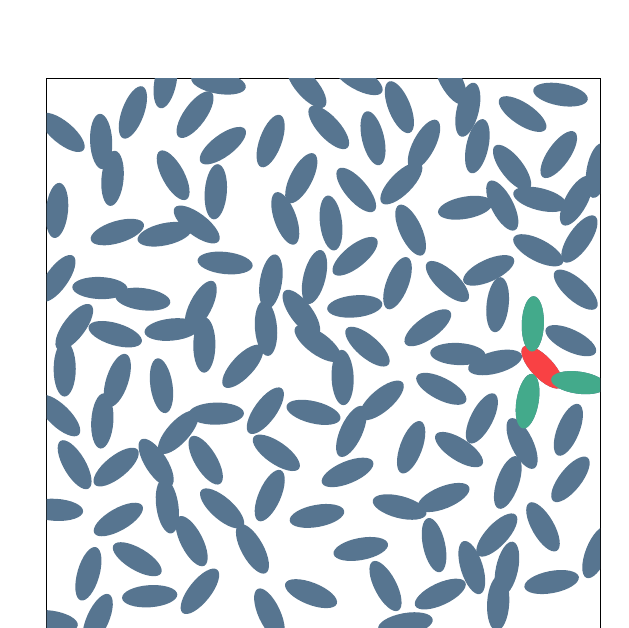
\begin{tikzpicture}

\definecolor{darkgray176}{RGB}{176,176,176}
\definecolor{gray}{RGB}{128,128,128}
\definecolor{steelblue31119180}{RGB}{31,119,180}

\begin{axis}[
    x=2, y=2,
    x grid style={darkgray176},
    xmin=0, xmax=100,
    y grid style={darkgray176},
    ymin=0, ymax=100,
    tick style={draw=none},
    yticklabels={,,},
    xtick
]
\draw[draw=none,fill=myblue,rotate around={260.204650150668:(axis cs:86.882913846962,41.6777189680256)}] (axis cs:86.882913846962,41.6777189680256) ellipse (5 and 2);
\draw[draw=none,fill=myblue,rotate around={352.916970683532:(axis cs:17.3702053810315,60.1099457262999)}] (axis cs:17.3702053810315,60.1099457262999) ellipse (5 and 2);
\draw[draw=none,fill=myblue,rotate around={22.6137910135262:(axis cs:54.3578505168292,28.8121800265779)}] (axis cs:54.3578505168292,28.8121800265779) ellipse (5 and 2);
\draw[draw=none,fill=myblue,rotate around={54.1605172415885:(axis cs:26.8061313592254,93.4547820902352)}] (axis cs:26.8061313592254,93.4547820902352) ellipse (5 and 2);
\draw[draw=none,fill=myblue,rotate around={349.787045848476:(axis cs:92.8377033572501,97.06536507931)}] (axis cs:92.8377033572501,97.06536507931) ellipse (5 and 2);
\draw[draw=none,fill=myblue,rotate around={301.169459612978:(axis cs:28.7329585023873,31.0188006699616)}] (axis cs:28.7329585023873,31.0188006699616) ellipse (5 and 2);
\draw[draw=none,fill=myblue,rotate around={9.99665572168897:(axis cs:64.8146228143106,1.40202864166694)}] (axis cs:64.8146228143106,1.40202864166694) ellipse (5 and 2);
\draw[draw=none,fill=myblue,rotate around={75.9590718992238:(axis cs:48.3915146177629,64.1181420805372)}] (axis cs:48.3915146177629,64.1181420805372) ellipse (5 and 2);
\draw[draw=none,fill=myblue,rotate around={227.038747519095:(axis cs:81.3272540913949,17.500793155944)}] (axis cs:81.3272540913949,17.500793155944) ellipse (5 and 2);
\draw[draw=none,fill=myblue,rotate around={248.168331406681:(axis cs:99.3939573851162,14.3982292725168)}] (axis cs:99.3939573851162,14.3982292725168) ellipse (5 and 2);
\draw[draw=none,fill=myblue,rotate around={190.315288515932:(axis cs:75.6429101109758,76.6325837014612)}] (axis cs:75.6429101109758,76.6325837014612) ellipse (5 and 2);
\draw[draw=none,fill=myblue,rotate around={52.992867030674:(axis cs:4.98633355030644,55.0858130674453)}] (axis cs:4.98633355030644,55.0858130674453) ellipse (5 and 2);
\draw[draw=none,fill=myblue,rotate around={54.0037365377994:(axis cs:39.5055460595019,39.9625444177252)}] (axis cs:39.5055460595019,39.9625444177252) ellipse (5 and 2);
\draw[draw=none,fill=myblue,rotate around={332.863827568311:(axis cs:71.3013949179524,43.9153887693566)}] (axis cs:71.3013949179524,43.9153887693566) ellipse (5 and 2);
\draw[draw=none,fill=myblue,rotate around={84.5473125880316:(axis cs:1.86286810442203,76.1448652422809)}] (axis cs:1.86286810442203,76.1448652422809) ellipse (5 and 2);
\draw[draw=none,fill=myblue,rotate around={294.754598975761:(axis cs:40.2510821396431,3.23948125486693)}] (axis cs:40.2510821396431,3.23948125486693) ellipse (5 and 2);
\draw[draw=none,fill=myblue,rotate around={353.860974913289:(axis cs:32.2412530863386,66.6502536503754)}] (axis cs:32.2412530863386,66.6502536503754) ellipse (5 and 2);
\draw[draw=none,fill=myblue,rotate around={268.079369117024:(axis cs:87.8331224981219,55.6504236167273)}] (axis cs:87.8331224981219,55.6504236167273) ellipse (5 and 2);
\draw[draw=none,fill=myblue,rotate around={249.914628955572:(axis cs:40.4644776697715,88.6819898491135)}] (axis cs:40.4644776697715,88.6819898491135) ellipse (5 and 2);
\draw[draw=none,fill=myblue,rotate around={315.9419617351:(axis cs:2.21483365114915,39.0946442609324)}] (axis cs:2.21483365114915,39.0946442609324) ellipse (5 and 2);
\draw[draw=none,fill=myblue,rotate around={29.7482081236702:(axis cs:12.948532403687,20.3052301632043)}] (axis cs:12.948532403687,20.3052301632043) ellipse (5 and 2);
\draw[draw=none,fill=myblue,rotate around={245.9296477557:(axis cs:9.21255957094804,2.22727254610813)}] (axis cs:9.21255957094804,2.22727254610813) ellipse (5 and 2);
\draw[draw=none,fill=myblue,rotate around={10.5803347867585:(axis cs:56.7525384036258,14.9822704642782)}] (axis cs:56.7525384036258,14.9822704642782) ellipse (5 and 2);
\draw[draw=none,fill=myblue,rotate around={231.67969665037:(axis cs:94.6296514046673,27.5593228059429)}] (axis cs:94.6296514046673,27.5593228059429) ellipse (5 and 2);
\draw[draw=none,fill=myblue,rotate around={246.320529683567:(axis cs:40.2988588854947,24.6222243618935)}] (axis cs:40.2988588854947,24.6222243618935) ellipse (5 and 2);
\draw[draw=none,fill=myblue,rotate around={345.812285412304:(axis cs:89.1671087210519,78.1531769002003)}] (axis cs:89.1671087210519,78.1531769002003) ellipse (5 and 2);
\draw[draw=none,fill=myblue,rotate around={319.270432431842:(axis cs:57.9576260069661,51.5378189312098)}] (axis cs:57.9576260069661,51.5378189312098) ellipse (5 and 2);
\draw[draw=none,fill=myblue,rotate around={98.5717374651543:(axis cs:20.7427655078686,44.4798361153012)}] (axis cs:20.7427655078686,44.4798361153012) ellipse (5 and 2);
\draw[draw=none,fill=myblue,rotate around={320.301578164404:(axis cs:2.81441707119023,90.2466579598913)}] (axis cs:2.81441707119023,90.2466579598913) ellipse (5 and 2);
\draw[draw=none,fill=myblue,rotate around={76.4647671337003:(axis cs:76.0905857450005,94.3357690743821)}] (axis cs:76.0905857450005,94.3357690743821) ellipse (5 and 2);
\draw[draw=none,fill=myblue,rotate around={84.9272953979372:(axis cs:11.9019594584809,81.9433638347379)}] (axis cs:11.9019594584809,81.9433638347379) ellipse (5 and 2);
\draw[draw=none,fill=myblue,rotate around={204.607367274743:(axis cs:79.8625822264079,65.311187764344)}] (axis cs:79.8625822264079,65.311187764344) ellipse (5 and 2);
\draw[draw=none,fill=myblue,rotate around={12.3739793687086:(axis cs:21.323586325317,71.8427228400097)}] (axis cs:21.323586325317,71.8427228400097) ellipse (5 and 2);
\draw[draw=none,fill=myblue,rotate around={117.168001814191:(axis cs:26.195767740668,16.3937377096593)}] (axis cs:26.195767740668,16.3937377096593) ellipse (5 and 2);
\draw[draw=none,fill=myblue,rotate around={274.460391494636:(axis cs:39.6281320324819,54.8484672789167)}] (axis cs:39.6281320324819,54.8484672789167) ellipse (5 and 2);
\draw[draw=none,fill=myblue,rotate around={130.54913502052:(axis cs:55.933435835093,79.8429238370018)}] (axis cs:55.933435835093,79.8429238370018) ellipse (5 and 2);
\draw[draw=none,fill=myblue,rotate around={132.433882308199:(axis cs:50.9653840442826,91.1428552378015)}] (axis cs:50.9653840442826,91.1428552378015) ellipse (5 and 2);
\draw[draw=none,fill=myblue,rotate around={69.0335688009109:(axis cs:63.3896028126425,63.0007610550364)}] (axis cs:63.3896028126425,63.0007610550364) ellipse (5 and 2);
\draw[draw=none,fill=myblue,rotate around={3.85375435108094:(axis cs:18.6121409896952,6.44416862770173)}] (axis cs:18.6121409896952,6.44416862770173) ellipse (5 and 2);
\draw[draw=none,fill=myblue,rotate around={242.14725970489:(axis cs:68.1720522704402,88.0252489706398)}] (axis cs:68.1720522704402,88.0252489706398) ellipse (5 and 2);
\draw[draw=none,fill=myblue,rotate around={289.801943190306:(axis cs:43.1108191914449,74.7060050602938)}] (axis cs:43.1108191914449,74.7060050602938) ellipse (5 and 2);
\draw[draw=none,fill=myblue,rotate around={282.464320644406:(axis cs:69.9923435700512,15.6729689301564)}] (axis cs:69.9923435700512,15.6729689301564) ellipse (5 and 2);
\draw[draw=none,fill=myblue,rotate around={234.724822456551:(axis cs:1.89041207297357,63.8556494308399)}] (axis cs:1.89041207297357,63.8556494308399) ellipse (5 and 2);
\draw[draw=none,fill=myblue,rotate around={302.616093260557:(axis cs:19.772606026042,30.5471205146096)}] (axis cs:19.772606026042,30.5471205146096) ellipse (5 and 2);
\draw[draw=none,fill=myblue,rotate around={158.340760048643:(axis cs:47.7631607343279,6.91010886104096)}] (axis cs:47.7631607343279,6.91010886104096) ellipse (5 and 2);
\draw[draw=none,fill=myblue,rotate around={202.054523659658:(axis cs:71.7026363458189,24.2772963730362)}] (axis cs:71.7026363458189,24.2772963730362) ellipse (5 and 2);
\draw[draw=none,fill=myblue,rotate around={69.6380570029668:(axis cs:15.5768836156765,93.8502782854917)}] (axis cs:15.5768836156765,93.8502782854917) ellipse (5 and 2);
\draw[draw=none,fill=myblue,rotate around={152.575999415476:(axis cs:88.8183765619847,68.9473725156417)}] (axis cs:88.8183765619847,68.9473725156417) ellipse (5 and 2);
\draw[draw=none,fill=myblue,rotate around={86.6229821231618:(axis cs:81.5765245617972,5.2010753658165)}] (axis cs:81.5765245617972,5.2010753658165) ellipse (5 and 2);
\draw[draw=none,fill=myblue,rotate around={69.5870529278177:(axis cs:65.8506228342984,33.3603805241784)}] (axis cs:65.8506228342984,33.3603805241784) ellipse (5 and 2);
\draw[draw=none,fill=myblue,rotate around={89.4563598649543:(axis cs:28.4867819268627,51.8325293958749)}] (axis cs:28.4867819268627,51.8325293958749) ellipse (5 and 2);
\draw[draw=none,fill=myblue,rotate around={118.92867917955:(axis cs:37.1783840900199,15.0048162820745)}] (axis cs:37.1783840900199,15.0048162820745) ellipse (5 and 2);
\draw[draw=none,fill=myblue,rotate around={10.7885285332415:(axis cs:91.2306043988741,9.00705471851809)}] (axis cs:91.2306043988741,9.00705471851809) ellipse (5 and 2);
\draw[draw=none,fill=myblue,rotate around={70.766031758227:(axis cs:83.3116224870324,26.9941651840805)}] (axis cs:83.3116224870324,26.9941651840805) ellipse (5 and 2);
\draw[draw=none,fill=myblue,rotate around={35.6434088614135:(axis cs:68.8597459043663,54.9424041219192)}] (axis cs:68.8597459043663,54.9424041219192) ellipse (5 and 2);
\draw[draw=none,fill=myblue,rotate around={51.5476613473339:(axis cs:27.6855305634842,7.33028459895518)}] (axis cs:27.6855305634842,7.33028459895518) ellipse (5 and 2);
\draw[draw=none,fill=myblue,rotate around={346.299933178858:(axis cs:48.2056048404719,39.6634016751004)}] (axis cs:48.2056048404719,39.6634016751004) ellipse (5 and 2);
\draw[draw=none,fill=myblue,rotate around={265.618518135428:(axis cs:30.5569873761105,79.5161765830348)}] (axis cs:30.5569873761105,79.5161765830348) ellipse (5 and 2);
\draw[draw=none,fill=myblue,rotate around={103.45201055566:(axis cs:58.9588736685684,89.1863749433072)}] (axis cs:58.9588736685684,89.1863749433072) ellipse (5 and 2);
\draw[draw=none,fill=myblue,rotate around={220.502650942834:(axis cs:60.5080407877913,41.8210802578143)}] (axis cs:60.5080407877913,41.8210802578143) ellipse (5 and 2);
\draw[draw=none,fill=myblue,rotate around={218.80828811829:(axis cs:55.7205303388384,67.860496152752)}] (axis cs:55.7205303388384,67.860496152752) ellipse (5 and 2);
\draw[draw=none,fill=myblue,rotate around={150.520494903969:(axis cs:56.2460532738079,99.98891155317)}] (axis cs:56.2460532738079,99.98891155317) ellipse (5 and 2);
\draw[draw=none,fill=myblue,rotate around={54.8255110517293:(axis cs:92.5194453046932,86.236230748634)}] (axis cs:92.5194453046932,86.236230748634) ellipse (5 and 2);
\draw[draw=none,fill=myblue,rotate around={300.366524500867:(axis cs:5.04996349555212,30.2011265445795)}] (axis cs:5.04996349555212,30.2011265445795) ellipse (5 and 2);
\draw[draw=none,fill=myblue,rotate around={254.060351773917:(axis cs:7.53779290855019,10.5024775779718)}] (axis cs:7.53779290855019,10.5024775779718) ellipse (5 and 2);
\draw[draw=none,fill=myblue,rotate around={294.878692522367:(axis cs:65.7557552355382,72.5896944885608)}] (axis cs:65.7557552355382,72.5896944885608) ellipse (5 and 2);
\draw[draw=none,fill=myblue,rotate around={16.7930611338574:(axis cs:12.7640613253374,72.239375523327)}] (axis cs:12.7640613253374,72.239375523327) ellipse (5 and 2);
\draw[draw=none,fill=myblue,rotate around={86.396868066909:(axis cs:10.0538312195155,38.1153271806579)}] (axis cs:10.0538312195155,38.1153271806579) ellipse (5 and 2);
\draw[draw=none,fill=myblue,rotate around={324.027291154328:(axis cs:49.0019491046676,52.1085809997291)}] (axis cs:49.0019491046676,52.1085809997291) ellipse (5 and 2);
\draw[draw=none,fill=myblue,rotate around={67.9654909980869:(axis cs:94.255974386524,36.5108506935766)}] (axis cs:94.255974386524,36.5108506935766) ellipse (5 and 2);
\draw[draw=none,fill=myblue,rotate around={251.941321158686:(axis cs:12.763648487112,45.4459238854269)}] (axis cs:12.763648487112,45.4459238854269) ellipse (5 and 2);
\draw[draw=none,fill=myblue,rotate around={190.351190759998:(axis cs:48.833234251249,20.9506374190798)}] (axis cs:48.833234251249,20.9506374190798) ellipse (5 and 2);
\draw[draw=none,fill=myblue,rotate around={298.612113224356:(axis cs:22.8495523863503,82.5045499767124)}] (axis cs:22.8495523863503,82.5045499767124) ellipse (5 and 2);
\draw[draw=none,fill=myblue,rotate around={352.400434801704:(axis cs:96.1055748110164,45.0288993232664)}] (axis cs:96.1055748110164,45.0288993232664) ellipse (5 and 2);
\draw[draw=none,fill=myblue,rotate around={24.9758141740133:(axis cs:71.1141108281389,6.83262257865851)}] (axis cs:71.1141108281389,6.83262257865851) ellipse (5 and 2);
\draw[draw=none,fill=myblue,rotate around={47.1120904509369:(axis cs:35.4257600506402,47.9798120950139)}] (axis cs:35.4257600506402,47.9798120950139) ellipse (5 and 2);
\draw[draw=none,fill=myblue,rotate around={14.7746567560795:(axis cs:81.0140107259634,48.6829084944324)}] (axis cs:81.0140107259634,48.6829084944324) ellipse (5 and 2);
\draw[draw=none,fill=myblue,rotate around={307.896545207601:(axis cs:84.0823937105312,83.8764630495301)}] (axis cs:84.0823937105312,83.8764630495301) ellipse (5 and 2);
\draw[draw=none,fill=myblue,rotate around={185.319571851166:(axis cs:55.6619378201471,58.8078579678459)}] (axis cs:55.6619378201471,58.8078579678459) ellipse (5 and 2);
\draw[draw=none,fill=myblue,rotate around={325.172336062301:(axis cs:41.4907403776405,32.3506445488188)}] (axis cs:41.4907403776405,32.3506445488188) ellipse (5 and 2);
\draw[draw=none,fill=myblue,rotate around={119.872128201725:(axis cs:89.6719005334523,18.9791507390857)}] (axis cs:89.6719005334523,18.9791507390857) ellipse (5 and 2);
\draw[draw=none,fill=myblue,rotate around={357.821530747641:(axis cs:9.62782038925507,62.1232922938803)}] (axis cs:9.62782038925507,62.1232922938803) ellipse (5 and 2);
\draw[draw=none,fill=myblue,rotate around={326.408690547729:(axis cs:85.9872570382636,93.5585714150404)}] (axis cs:85.9872570382636,93.5585714150404) ellipse (5 and 2);
\draw[draw=none,fill=myblue,rotate around={165.491621211313:(axis cs:63.768546413739,22.5593396318724)}] (axis cs:63.768546413739,22.5593396318724) ellipse (5 and 2);
\draw[draw=none,fill=myblue,rotate around={62.5689723853916:(axis cs:45.999869632787,81.9718303639362)}] (axis cs:45.999869632787,81.9718303639362) ellipse (5 and 2);
\draw[draw=none,fill=myblue,rotate around={80.686868301937:(axis cs:40.513972119891,63.2574647102097)}] (axis cs:40.513972119891,63.2574647102097) ellipse (5 and 2);
\draw[draw=none,fill=myblue,rotate around={352.160175168487:(axis cs:0.670179449571862,1.8587023245636)}] (axis cs:0.670179449571862,1.8587023245636) ellipse (5 and 2);
\draw[draw=none,fill=myblue,rotate around={147.152087004351:(axis cs:74.5059127687272,32.94117457168)}] (axis cs:74.5059127687272,32.94117457168) ellipse (5 and 2);
\draw[draw=none,fill=myblue,rotate around={79.912177589682:(axis cs:99.5409900854364,83.3507452903862)}] (axis cs:99.5409900854364,83.3507452903862) ellipse (5 and 2);
\draw[draw=none,fill=myblue,rotate around={0.893218153011031:(axis cs:30.6413648667477,39.4308194959482)}] (axis cs:30.6413648667477,39.4308194959482) ellipse (5 and 2);
\draw[draw=none,fill=myblue,rotate around={149.39430802483:(axis cs:16.364079445829,13.1332597438818)}] (axis cs:16.364079445829,13.1332597438818) ellipse (5 and 2);
\draw[draw=none,fill=myblue,rotate around={263.614140785283:(axis cs:81.4779667377777,59.1129447486611)}] (axis cs:81.4779667377777,59.1129447486611) ellipse (5 and 2);
\draw[draw=none,fill=myblue,rotate around={356.776002302174:(axis cs:1.58847438749508,22.0501701614518)}] (axis cs:1.58847438749508,22.0501701614518) ellipse (5 and 2);
\draw[draw=none,fill=myblue,rotate around={170.091144245238:(axis cs:31.0423654417477,99.2149038897966)}] (axis cs:31.0423654417477,99.2149038897966) ellipse (5 and 2);
\draw[draw=none,fill=myblue,rotate around={130.754835632223:(axis cs:46.9468771825903,98.6594198824206)}] (axis cs:46.9468771825903,98.6594198824206) ellipse (5 and 2);
\draw[draw=none,fill=myblue,rotate around={177.160830537073:(axis cs:74.2938016624452,50.2051842249504)}] (axis cs:74.2938016624452,50.2051842249504) ellipse (5 and 2);
\draw[draw=none,fill=myblue,rotate around={242.728282134562:(axis cs:78.6279318778352,38.5714724755397)}] (axis cs:78.6279318778352,38.5714724755397) ellipse (5 and 2);
\draw[draw=none,fill=myblue,rotate around={92.6718119634767:(axis cs:9.83995614919241,88.6061914819749)}] (axis cs:9.83995614919241,88.6061914819749) ellipse (5 and 2);
\draw[draw=none,fill=myblue,rotate around={154.348461856241:(axis cs:94.6984370754419,52.6195822773216)}] (axis cs:94.6984370754419,52.6195822773216) ellipse (5 and 2);
\draw[draw=none,fill=myblue,rotate around={163.428804825857:(axis cs:12.3813878424189,53.7827644674075)}] (axis cs:12.3813878424189,53.7827644674075) ellipse (5 and 2);
\draw[draw=none,fill=myblue,rotate around={242.708068430962:(axis cs:27.8300822695283,58.8917633929874)}] (axis cs:27.8300822695283,58.8917633929874) ellipse (5 and 2);
\draw[draw=none,fill=myblue,rotate around={235.475628484884:(axis cs:96.2473706632951,70.984470876944)}] (axis cs:96.2473706632951,70.984470876944) ellipse (5 and 2);
\draw[draw=none,fill=myblue,rotate around={36.656268675175:(axis cs:31.8306870443883,87.8458564448473)}] (axis cs:31.8306870443883,87.8458564448473) ellipse (5 and 2);
\draw[draw=none,fill=myblue,rotate around={112.043249573373:(axis cs:63.7252837899546,94.8004298199742)}] (axis cs:63.7252837899546,94.8004298199742) ellipse (5 and 2);
\draw[draw=none,fill=myblue,rotate around={92.0523885815362:(axis cs:53.4661151748034,45.9549267427767)}] (axis cs:53.4661151748034,45.9549267427767) ellipse (5 and 2);
\draw[draw=none,fill=myblue,rotate around={245.449379453127:(axis cs:55.0511046066284,36.2202640673709)}] (axis cs:55.0511046066284,36.2202640673709) ellipse (5 and 2);
\draw[draw=none,fill=myblue,rotate around={295.652389779659:(axis cs:85.8883818155678,34.0384614709201)}] (axis cs:85.8883818155678,34.0384614709201) ellipse (5 and 2);
\draw[draw=none,fill=myblue,rotate around={225.194198562187:(axis cs:64.0823849056176,81.0403814957276)}] (axis cs:64.0823849056176,81.0403814957276) ellipse (5 and 2);
\draw[draw=none,fill=myblue,rotate around={96.995820274412:(axis cs:51.3744048894096,73.8743045476509)}] (axis cs:51.3744048894096,73.8743045476509) ellipse (5 and 2);
\draw[draw=none,fill=myblue,rotate around={98.0898695872326:(axis cs:21.8022369733386,22.7350748099463)}] (axis cs:21.8022369733386,22.7350748099463) ellipse (5 and 2);
\draw[draw=none,fill=myblue,rotate around={138.78854758218:(axis cs:31.6959886698282,22.3058845988067)}] (axis cs:31.6959886698282,22.3058845988067) ellipse (5 and 2);
\draw[draw=none,fill=myblue,rotate around={318.492823597775:(axis cs:95.5877271140043,61.8264497134761)}] (axis cs:95.5877271140043,61.8264497134761) ellipse (5 and 2);
\draw[draw=none,fill=myblue,rotate around={259.231220358722:(axis cs:21.4771599692152,99.5192993241954)}] (axis cs:21.4771599692152,99.5192993241954) ellipse (5 and 2);
\draw[draw=none,fill=myblue,rotate around={269.741531872192:(axis cs:3.25648736233763,47.5197410511917)}] (axis cs:3.25648736233763,47.5197410511917) ellipse (5 and 2);
\draw[draw=none,fill=myblue,rotate around={297.353285854387:(axis cs:61.218038462067,8.28676729492537)}] (axis cs:61.218038462067,8.28676729492537) ellipse (5 and 2);
\draw[draw=none,fill=myblue,rotate around={47.726999713751:(axis cs:23.780568342442,36.0723097613012)}] (axis cs:23.780568342442,36.0723097613012) ellipse (5 and 2);
\draw[draw=none,fill=myblue,rotate around={77.7238081358585:(axis cs:83.1646923435251,11.4032470035099)}] (axis cs:83.1646923435251,11.4032470035099) ellipse (5 and 2);
\draw[draw=none,fill=myblue,rotate around={317.080766857636:(axis cs:72.4044215935182,63.3080070150894)}] (axis cs:72.4044215935182,63.3080070150894) ellipse (5 and 2);
\draw[draw=none,fill=myblue,rotate around={38.7891838094475:(axis cs:12.5489499377054,29.7759902549972)}] (axis cs:12.5489499377054,29.7759902549972) ellipse (5 and 2);
\draw[draw=none,fill=myblue,rotate around={313.711203512664:(axis cs:89.5227528142594,47.8325968256834)}] (axis cs:89.5227528142594,47.8325968256834) ellipse (5 and 2);
\draw[draw=none,fill=myblue,rotate around={298.477328346312:(axis cs:72.9707250021413,99.7706074619335)}] (axis cs:72.9707250021413,99.7706074619335) ellipse (5 and 2);
\draw[draw=none,fill=myblue,rotate around={5.81423179660655:(axis cs:22.6543381808917,54.6284359265346)}] (axis cs:22.6543381808917,54.6284359265346) ellipse (5 and 2);
\draw[draw=none,fill=myblue,rotate around={107.369343119315:(axis cs:76.8084025367909,11.622625330049)}] (axis cs:76.8084025367909,11.622625330049) ellipse (5 and 2);
\draw[draw=none,fill=myblue,rotate around={297.410687409085:(axis cs:82.316163382063,77.0255989351747)}] (axis cs:82.316163382063,77.0255989351747) ellipse (5 and 2);
\draw[draw=none,fill=myblue,rotate around={241.412768220482:(axis cs:95.6908177165746,77.8990008145085)}] (axis cs:95.6908177165746,77.8990008145085) ellipse (5 and 2);
\draw[draw=none,fill=myblue,rotate around={306.721684207499:(axis cs:46.0121623420069,57.6240632220017)}] (axis cs:46.0121623420069,57.6240632220017) ellipse (5 and 2);
\draw[draw=none,fill=myblue,rotate around={322.736476985811:(axis cs:27.1112894933776,73.6073827622796)}] (axis cs:27.1112894933776,73.6073827622796) ellipse (5 and 2);
\draw[draw=none,fill=myblue,rotate around={77.4649729853431:(axis cs:77.8123782915191,87.7467385017039)}] (axis cs:77.8123782915191,87.7467385017039) ellipse (5 and 2);
\draw[draw=none,fill=myred,rotate around={313.711203512664:(axis cs:89.5227528142594,47.8325968256834)}] (axis cs:89.5227528142594,47.8325968256834) ellipse (5 and 2);
\draw[draw=none,fill=mygreen,rotate around={260.204650150668:(axis cs:86.882913846962,41.6777189680256)}] (axis cs:86.882913846962,41.6777189680256) ellipse (5 and 2);
\draw[draw=none,fill=mygreen,rotate around={268.079369117024:(axis cs:87.8331224981219,55.6504236167273)}] (axis cs:87.8331224981219,55.6504236167273) ellipse (5 and 2);
\draw[draw=none,fill=mygreen,rotate around={352.400434801704:(axis cs:96.1055748110164,45.0288993232664)}] (axis cs:96.1055748110164,45.0288993232664) ellipse (5 and 2);
\end{axis}

\end{tikzpicture}
}
    \caption{Prikaz porazdelitve~$128$ elips.
    Na sredinski sliki izberemo naključno elipso in pogledamo njeno okolico polmera 
    $2a$. Na zadnji sliki so označene samo še tiste elipse iz okolice s~katerimi 
    se izbrana elipsa prekriva.}
    \label{fig:zaznavanje_trkov}
\end{figure}

\section{Parametri sistema}
\subsection{Energija}
Sistemu definiramo prekrivalno enrgijo na sledeč način
\begin{equation}
    u = \sum_{i \neq j} \log{\mu_{i,j}^2} 
\end{equation}
%\input{zakljucek}

%------------------------------------------------------------------------
%       LITERATURA
%------------------------------------------------------------------------

\cleardoublepage
\renewcommand\bibname{Literatura}
\bibliographystyle{apsrev4-2-fmf-slo}
\bibliography{Bibliografija-slo}


%-----------------------------------------------------------------------
%       DODATKI
%-----------------------------------------------------------------------

\cleardoublepage\phantomsection
\titleformat{\chapter}[display]
{\bfseries\huge}{\chaptertitlename\ \thechapter}{1ex}{\huge\filright #1}


% \begin{appendices}   

%\input{Naslov prvega dodatka}
%\input{Naslov drugega dodatk}

% \end{appendices}


%-----------------------------------------------------------------------
%       KAZALO (NEOBVEZNO)
%-----------------------------------------------------------------------

% \cleardoublepage
% \printindex

\end{document}